% =====================================================================================
%  Thermal crosstalk as a resource: a few-heater, heat-spreading silicon optical phased array
%  EE798 (Nanophotonics) course project report, IIT Kanpur, November 2026
%
%  Build:  pdflatex report  ->  bibtex report  ->  pdflatex report  (twice)
%  On Overleaf: upload this folder as it is (report.tex, sections/, figures/, references.bib).
% =====================================================================================
\documentclass[11pt,a4paper]{article}

% ---------- encoding, fonts, page ------------------------------------------------------
\usepackage[T1]{fontenc}
\usepackage[utf8]{inputenc}
\usepackage{lmodern}
\usepackage{microtype}
\usepackage[a4paper,hmargin=29mm,vmargin=26mm,headheight=14pt]{geometry}   % 152 mm text width
\linespread{1.06}
\setlength{\parskip}{0.35\baselineskip plus 1pt}
\setlength{\parindent}{0pt}

% ---------- mathematics and units ------------------------------------------------------
\usepackage{amsmath,amssymb,bm}
\usepackage{siunitx}
\sisetup{
  per-mode            = symbol,
  range-phrase        = {--},
  range-units         = single,
  separate-uncertainty= true,
  detect-weight       = true,
  mode                = match,
  group-minimum-digits= 5,
}
\DeclareSIUnit\rad{rad}
\DeclareSIUnit\deg{deg}

% ---------- figures and tables ---------------------------------------------------------
\usepackage{graphicx}
\graphicspath{{figures/}}
\usepackage[font=small,labelfont=bf,labelsep=period,skip=6pt]{caption}
\usepackage{subcaption}
\usepackage{booktabs,tabularx,array,multirow,longtable,threeparttable}
\usepackage{float,placeins}
\usepackage{xcolor}
\usepackage{enumitem}
\setlist{itemsep=2pt,topsep=3pt,parsep=0pt,leftmargin=1.6em}
\renewcommand{\arraystretch}{1.15}
\newcolumntype{L}{>{\raggedright\arraybackslash}X}
\newcolumntype{P}[1]{>{\raggedright\arraybackslash}p{#1}}
\setlength{\textfloatsep}{14pt plus 2pt minus 2pt}
\setlength{\floatsep}{12pt plus 2pt minus 2pt}
\setlength{\intextsep}{12pt plus 2pt minus 2pt}
\renewcommand{\topfraction}{0.85}
\renewcommand{\bottomfraction}{0.7}
\renewcommand{\textfraction}{0.1}
\renewcommand{\floatpagefraction}{0.75}

% ---------- headings, header, appendix -------------------------------------------------
\usepackage{titlesec}
\titleformat{\section}{\Large\bfseries}{\thesection}{0.8em}{}
\titleformat{\subsection}{\large\bfseries}{\thesubsection}{0.8em}{}
\titleformat{\subsubsection}{\normalsize\bfseries}{\thesubsubsection}{0.8em}{}
\titlespacing*{\section}{0pt}{18pt plus 4pt minus 2pt}{6pt}
\titlespacing*{\subsection}{0pt}{13pt plus 3pt minus 2pt}{4pt}
\titlespacing*{\subsubsection}{0pt}{10pt plus 2pt minus 2pt}{3pt}
\usepackage{fancyhdr}
\pagestyle{fancy}
\fancyhf{}
\fancyhead[L]{\small\itshape Thermal crosstalk as a resource for optical phased arrays}
\fancyhead[R]{\small\thepage}
\renewcommand{\headrulewidth}{0.3pt}

% ---------- references and links -------------------------------------------------------
\usepackage[numbers,sort&compress]{natbib}
\setlength{\bibsep}{3pt plus 1pt}
\usepackage[colorlinks=true,linkcolor=blue!45!black,citecolor=blue!45!black,urlcolor=blue!45!black]{hyperref}
\usepackage{doi}
\usepackage[capitalise,noabbrev,nameinlink]{cleveref}
\crefname{equation}{Eq.}{Eqs.}
\Crefname{equation}{Equation}{Equations}
\crefname{appendix}{Appendix}{Appendices}

% ---------- project macros -------------------------------------------------------------
\newcommand{\neff}{n_{\mathrm{eff}}}
\newcommand{\dndT}{\mathrm{d}\neff/\mathrm{d}T}
\newcommand{\Ppi}{P_{\pi}}
\newcommand{\Lth}{L_{\mathrm{th}}}
\newcommand{\Lh}{L_{\mathrm{h}}}
\newcommand{\kt}{k\,t}
\newcommand{\xh}{x_{\mathrm{h}}}
\newcommand{\dd}{\mathrm{d}}
\newcommand{\ee}{\mathrm{e}}
\newcommand{\ii}{\mathrm{i}}
\newcommand{\est}{(est.)}
\newcommand{\mWdeg}{\milli\watt\per\deg}
\newcommand{\KmW}{\kelvin\metre\per\watt}        % temperature rise per W/m of heater power
\newcommand{\stack}[1]{\textsf{#1}}               % names of the four structures

\hypersetup{
  pdftitle  = {Thermal crosstalk as a resource: steering and focusing a silicon optical phased array with a few heaters},
  pdfauthor = {Shreyansh Mehta},
}

% =====================================================================================
\begin{document}

\begin{titlepage}
  \centering
  \vspace*{22mm}
  {\large EE798: Nanophotonics \quad$\cdot$\quad Course project report\par}
  \vspace{16mm}
  {\LARGE\bfseries Thermal crosstalk as a resource:\par}
  \vspace{3mm}
  {\Large\bfseries steering and focusing a silicon optical phased array\\[2pt] with a few heaters\par}
  \vspace{14mm}
  {\large Shreyansh Mehta\par}
  \vspace{2mm}
  {\normalsize Department of Physics, Indian Institute of Technology Kanpur\par}
  \vspace{2mm}
  {\normalsize November 2026\par}
  \vfill
\end{titlepage}

% ---------- abstract -------------------------------------------------------------------
\begin{abstract}
\noindent
Silicon optical phased arrays (OPAs) usually give each emitter its own heater and are designed so that heat does
not spread from one waveguide to the next. This report examines whether that spreading can be used instead,
so that $K$ heaters steer $N>K$ emitters. We model a silicon-on-insulator array of \num{33} emitters at
\qty{2}{\micro\metre} pitch and \qty{1550}{\nano\metre}, using verified COMSOL finite-element models for the
optics and heat flow and a Python model of the array for the far field and the heater optimisation.
Heat spreading acts as a spatial low-pass filter on the phase. On a standard stack it is too short-ranged for
few heaters to steer. On an oxide membrane suspended under the whole array, a slot past the edge heater forces
all the heat across the array and produces a linear phase ramp: three heaters steer \ang{22.8} at
\qty{1.38}{\mWdeg} in air, and in vacuum one heater does so at \qty{0.53}{\mWdeg}, within \qty{5}{\percent} of
a conduction limit that is independent of $N$. This is \numrange{10}{30} times below published few-wire arrays
at the same pitch, but \num{3.6} times above an array of the best published phase shifters at \ang{10}, because a
smooth ramp cannot be phase-wrapped. The same membrane forms a one-wire tunable lens at about
\qty{1}{\milli\watt\per\rad}. The costs are millisecond settling, which drives shaped independently for each heater shorten six to twelve
times, two to four usable phase patterns, a hottest
waveguide about \qty{62}{\kelvin} above ambient at \ang{10}, and the need for a one-time static trim of
fabrication errors.
\end{abstract}

\vspace{4mm}
{\small\tableofcontents}
\clearpage

% ---------- body -----------------------------------------------------------------------
% =====================================================================================
\section{Introduction}
\label{sec:intro}
% =====================================================================================

An optical phased array (OPA) splits a laser beam into coherent copies, sends each down its own waveguide and
emits each from a grating. The phase difference between neighbouring emitters sets the direction of the combined
beam across the array; the grating period and the wavelength set it along the other
axis~\cite{sun2013}. OPAs point beams without moving parts and are studied for LiDAR, free-space optical
links and biophotonic probes~\cite{hsu2022}.

In silicon the phases are usually set thermo-optically: a heater above a waveguide raises its refractive index and
delays the light. The conventional design gives each emitter its own heater and wire, and treats heat leaking to
neighbouring waveguides (thermal crosstalk) as a defect. It is suppressed by spacing the heaters
\qtyrange{15}{100}{\micro\metre} apart and converging the waveguides afterwards~\cite{phare2018,miller2020},
by trenches and undercuts~\cite{parsons2025,fang2011}, or by calibration. \Cref{fig:topview}(a) shows the result: $N$ heaters, $N$ wires and a fan-in region
whose only purpose is to keep the heaters apart.

\begin{figure}[htbp]
  \centering
  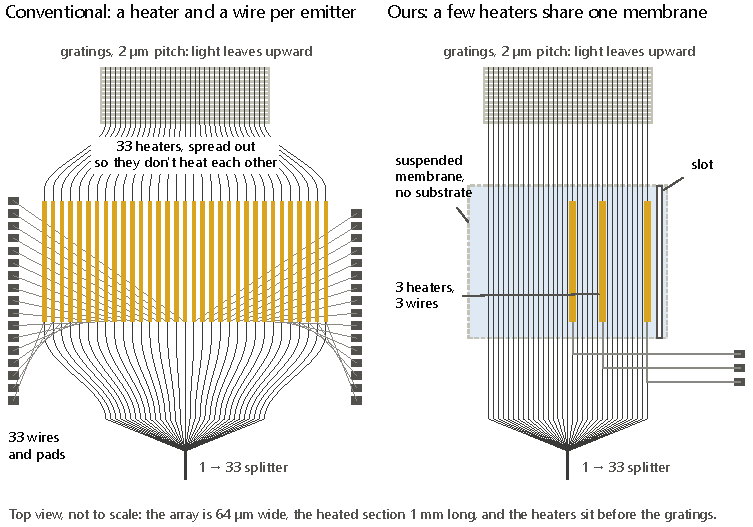
\includegraphics[width=\linewidth]{fig12_topview}
  \caption{A conventional thermo-optic OPA and the design studied here, seen from above (schematic). (a)~One
  heater, wire and pad per emitter, with the heaters spaced so that their heat does not overlap, and a fan-in to
  the emitter pitch. (b)~This work: the waveguides stay at the emitter pitch and cross a suspended oxide membrane
  before the gratings. One to three heaters set the phase of all \num{33} waveguides through the heat they share;
  a slot past the edge heater forces that heat to cross the array.}
  \label{fig:topview}
\end{figure}

Individual heaters provide three capabilities. (i)~\emph{Arbitrary patterns}: each emitter can take any phase, so
the array can form several beams or holograms. (ii)~\emph{Phase wrapping}: phase matters only modulo $2\pi$, so no
heater ever supplies more than $2\pi$. (iii)~\emph{Per-emitter calibration}: each waveguide's fabrication error can
be cancelled by its own heater.

Steering, however, needs only a smooth phase profile, a linear ramp across the array, and heat spreads smoothly.
This report therefore asks:
\begin{quote}
  With $K$ heaters driving $N>K$ emitters through shared heat, how well can the array steer and focus, and what
  does it cost in power, speed and control compared with one isolated heater per emitter?
\end{quote}

Steady heat conduction acts as a spatial low-pass filter on the phase: whatever the heaters supply is smoothed
over a spreading length $\Lth$. If $\Lth$ is shorter than the emitter pitch $d$, each heater addresses one emitter,
which is the conventional design. If $\Lth\gg d$, a few heaters reach every emitter, but only smooth profiles can
be made (an offset, a ramp, a dome). Two consequences follow immediately. A ramp cannot be wrapped, so it must be
built in full: at \ang{10} the last emitter must lead the first by \qty{45}{\rad}. And independent fabrication
errors, the sharpest pattern of all, cannot be corrected. The ratio $\Lth/d$, set by the layer structure, decides
the regime.

\paragraph{Approach.} The study is simulation only (\cref{fig:pipeline}). COMSOL finite-element models supply the
physics: the waveguide mode and its thermo-optic coefficient, the optical coupling between waveguides, the
steady and transient temperature that one heater produces at every waveguide, the grating emission, and the limit
of the linear thermal model (\cref{sec:models}). Each is checked for convergence, energy balance and consistency
(\cref{sec:verification}). Because heat conduction is linear, the phases are a matrix product of the COMSOL
profiles and the heater powers; a Python model built on this, and checked against analytic limits, searches
thousands of heater layouts (\cref{sec:methods}).

\paragraph{Main results.}
\begin{enumerate}
  \item On a standard stack, heat sinks into the substrate within \qty{3.3}{\micro\metre}, and few heaters cannot
        steer. On an oxide membrane suspended under the whole array, three to four heaters steer
        \ang{\pm 16}--\ang{22.8} at about \qty{4.9}{\mWdeg}.
  \item A slot cut past the edge heater forces all its heat to cross the array, which makes the temperature a
        straight ramp. Three heaters then steer \ang{22.8} at \qty{1.38}{\mWdeg}; in vacuum one heater does so at
        \qty{0.53}{\mWdeg}, within \qty{5}{\percent} of a conduction limit that is independent of $N$.
  \item This is \numrange{10}{30} times below published few-wire arrays. Because the ramp cannot be wrapped,
        however, \num{33} of the best published folded phase shifters would need \num{3.6} times less power at
        \ang{10}.
  \item All three capabilities of individual control are lost, and each loss is quantified: two to four usable
        phase patterns, no correction of independent fabrication errors (so a one-time trim is required), and a
        hottest waveguide about \qty{62}{\kelvin} above ambient at \ang{10}.
  \item A \ang{10} step settles in \qtyrange{2}{9}{\milli\second} with a plain step drive. Because the heaters are
        few and independent, their drives can be shaped in time (pre-emphasis), which shortens this six to
        twelve times at three times the hold power.
  \item A uniformly heated membrane between two walls has a parabolic temperature profile, so one heater forms a
        tunable cylindrical lens at about \qty{1.2}{\milli\watt\per\rad}.
\end{enumerate}

To our knowledge, this is the first design study to use lateral heat spreading from one to five heaters as the
main steering and focusing actuator, with the membrane shaped to make the profile linear (\cref{sec:related}).

\Cref{sec:background} gives the theory, \cref{sec:models,sec:methods} the models, and \cref{sec:verification} the
checks. \Cref{sec:steering} presents the steering results and \cref{sec:other} the remaining properties.
\Cref{sec:discussion} compares with published devices and lists the limitations.

% =====================================================================================
\section{Background and theory}
\label{sec:background}
% =====================================================================================

\subsection{From phases to a beam}
\label{sec:arraytheory}

For $N$ identical emitters at positions $x_n$ with pitch $d$, equal amplitudes and phases $\phi_n$, the far-field
intensity at angle $\theta$ from the surface normal is
\begin{equation}
  I(\theta) \;=\; \mathrm{EP}(\theta)\,\Bigl|\frac{1}{N}\sum_{n=1}^{N} \ee^{\,\ii(\phi_n - k_0 x_n \sin\theta)}\Bigr|^{2},
  \qquad k_0=\frac{2\pi}{\lambda},
  \label{eq:farfield}
\end{equation}
where $\mathrm{EP}(\theta)$ is the single-emitter (element) pattern and $\lambda$ the free-space wavelength.

\paragraph{Steering.} A linear ramp $\phi_n=n\,\Delta\phi$ points the beam at
\begin{equation}
  \sin\theta_0 \;=\; \frac{\Delta\phi\,\lambda}{2\pi d}
  \label{eq:steer}
\end{equation}
(\cref{fig:basics}a). Only the step between neighbours matters; a common offset changes nothing and is left free
throughout.

\paragraph{Field of view.} The pattern repeats when $\sin\theta$ shifts by $\lambda/d$, producing grating lobes. A
single beam is obtained for $|\Delta\phi|\le\pi$, that is,
\begin{equation}
  |\theta_0| \;\le\; \arcsin\frac{\lambda}{2d} \;=\; \ang{22.8}
  \qquad(\lambda=\qty{1.55}{\micro\metre},\ d=\qty{2}{\micro\metre}).
  \label{eq:fov}
\end{equation}
At this pitch the nearest grating lobe is only \qty{2.4}{\decibel} below the main beam. Every
\qty{2}{\micro\metre}-pitch array has this limitation, regardless of how the phases are set, so side-lobe
suppression cannot distinguish between designs. We therefore use the Strehl ratio (\cref{sec:metrics}) as the
measure of beam quality. The \qty{66}{\micro\metre} aperture gives a beam \ang{1.2} wide (FWHM), so the field holds
about \num{34} resolvable spots.

\paragraph{Focusing.} A parabolic phase with the centre leading the edges focuses the light to a line at
distance $f$ (\cref{fig:basics}b). In the paraxial limit
\begin{equation}
  \phi(x) \;=\; c - \frac{k_0 x^{2}}{2f},
  \qquad
  a \;\equiv\; \phi(0)-\phi(X) \;=\; \frac{k_0 X^{2}}{2f},
  \label{eq:lens}
\end{equation}
where $X=\qty{32}{\micro\metre}$ is the half-aperture and $a$ the \emph{lens strength}. For this array
$a\,f=\qty{2076}{\rad\,\micro\metre}$, so $a=\qty{1}{\rad}$ corresponds to $f=\qty{2.1}{\milli\metre}$.

\begin{figure}[htbp]
  \centering
  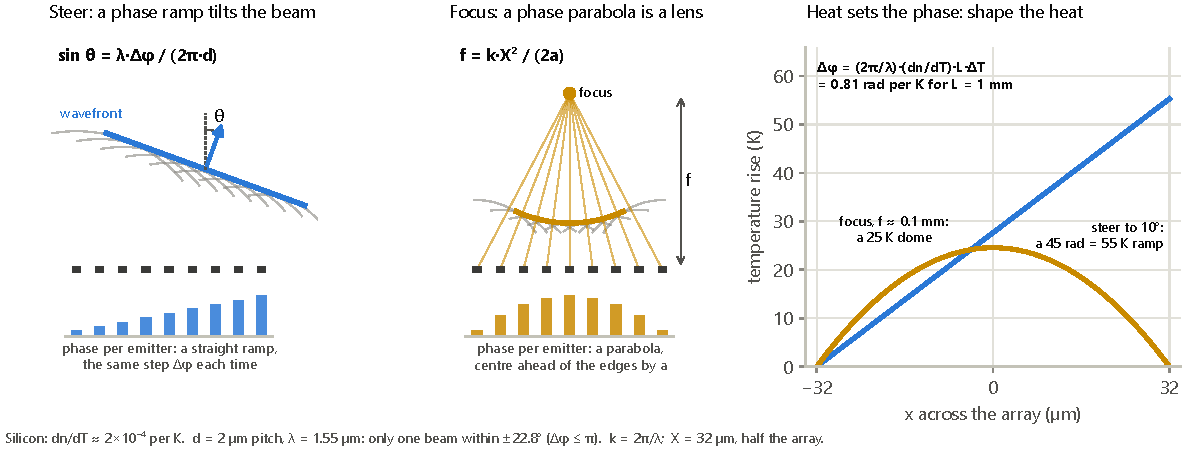
\includegraphics[width=\linewidth]{fig15_opa_basics}
  \caption{Steering and focusing (schematic, nine emitters). (a)~A linear phase ramp tilts the wavefront:
  $\sin\theta=\lambda\Delta\phi/(2\pi d)$. (b)~A parabolic phase focuses at $f=k_0X^2/(2a)$. (c)~The phase follows
  the temperature, \qty{0.81}{\rad\per\kelvin} for a \qty{1}{\milli\metre} heater, so the temperature must have the
  shape of the required phase. Shown: the \ang{10} ramp (\qty{45}{\rad}, \qty{55}{\kelvin} across the array) and a
  \qty{20}{\rad} lens.}
  \label{fig:basics}
\end{figure}

\subsection{From heat to phase}
\label{sec:heatphase}

A waveguide section of length $\Lh$ heated by $\Delta T$ delays its light by
\begin{equation}
  \phi \;=\; k_0\,\frac{\dd\neff}{\dd T}\,\Delta T\,\Lh ,
  \label{eq:phaseT}
\end{equation}
where $\neff$ is the effective index of the mode. For our waveguide $\dndT=\qty{2.009e-4}{\per\kelvin}$
(\cref{sec:modelA}), so a $2\pi$ shift needs \qty{7.7}{\kelvin\milli\metre}.

The heaters are much longer than the layer stack is thick, so temperature is computed in the cross-section, per
unit length. A heater at $\xh$ dissipating $P/\Lh$ per unit length raises the core at $x$ by
$\Delta T(x)=R(x;\xh)\,P/\Lh$, where $R$, the \emph{thermal kernel}, is in \unit{\KmW}. Substituting into
\cref{eq:phaseT}, the heater length cancels:
\begin{equation}
  \phi(x) \;=\; \gamma\,R(x;\xh)\,P,
  \qquad \gamma \equiv k_0\,\frac{\dd\neff}{\dd T} = \qty{814.4}{\rad\per\kelvin\per\metre}.
  \label{eq:phaseP}
\end{equation}
The phase depends only on total heater power. The length sets the temperature, $\Delta T=\phi/(\gamma\Lh)$, and
therefore enters only as a constraint. For the core under a heater, the power for a phase of $\pi$ is
\begin{equation}
  \Ppi \;=\; \frac{\pi}{\gamma\,R(\xh;\xh)} ,
  \label{eq:Ppi}
\end{equation}
so a lower $\Ppi$ requires a larger thermal resistance from the core to the heat sink. That resistance, together
with the heat capacity of the heated material, also sets the response time, so power and speed trade against each
other.

\subsection{Several heaters: superposition}
\label{sec:superposition}

For $K$ heaters at $x_k$ with powers $P_k$, the phase at emitter $n$ is taken as the sum of the single-heater
contributions,
\begin{equation}
  \phi_n \;=\; \sum_{k=1}^{K} G_{nk}\,P_k,
  \qquad
  G_{nk} \;=\; \gamma\,R(x_n;x_k),
  \label{eq:G}
\end{equation}
or $\bm\phi=G\bm P$. This step underlies every result in the report, so we justify it.

\paragraph{Proof.} Let $u=T-T_0$ be the temperature rise. With temperature-independent conductivity $k(\bm r)$,
the steady temperature satisfies
\begin{equation}
  \mathcal L u \;\equiv\; -\nabla\!\cdot\!\bigl(k\,\nabla u\bigr) \;=\; q(\bm r),
  \label{eq:heat}
\end{equation}
with $u=0$ on the substrate bottom and $\bm n\cdot k\nabla u=0$ on all other boundaries,
where $q=\sum_k q_k$ is the heat generated by all heaters. Let $u_k$ solve \cref{eq:heat} with heater $k$ alone.
The operator $\mathcal L$ is linear and both boundary conditions are homogeneous, so $u_\Sigma=\sum_k u_k$ satisfies
$\mathcal L u_\Sigma=\sum_k q_k=q$ and the same boundary conditions. The solution of \cref{eq:heat} is unique: if
$u_1$ and $u_2$ both solve it, their difference $w$ obeys $\mathcal Lw=0$ with the same homogeneous conditions, and
multiplying by $w$ and integrating by parts gives $\int k\,|\nabla w|^2\,\dd A=0$, so $w$ is constant and, since
$w=0$ on the substrate bottom, zero. Hence $u=\sum_k u_k$ exactly. Each $u_k$ scales linearly with $P_k$, and the
phase is linear in temperature (\cref{eq:phaseT}, confirmed to \qty{0.3}{\percent} by a coupled mode solve in
\cref{sec:comsolchecks}), which gives \cref{eq:G}. The same argument applies to the time-dependent equation, so
step responses also superpose.

\paragraph{Where it fails, and by how much.} Superposition requires $k$ independent of temperature. In reality
oxide conducts slightly better and silicon slightly worse when hot. The thermal model was therefore run with
temperature-dependent conductivities and two heaters \qty{6}{\micro\metre} apart, each alone and both together,
for both stacks (\cref{sec:modelF}). At peak rises of \qty{115}{\kelvin} (standard stack) and \qty{177}{\kelvin}
(undercut), the sum of the single-heater profiles exceeds the two-heater solution by \qty{1.7}{\percent} and
\qty{2.8}{\percent} of the peak. This discrepancy is fully explained by the temperature dependence: after the
Kirchhoff transform of \cref{sec:nonlinear}, the residual is \qty{0.08}{\percent} and \qty{0.14}{\percent}. Using
the same transform, the error of plain superposition for the slot design at \ang{10} with \qty{1}{\milli\metre}
heaters (peak \qty{63}{\kelvin}) is \qty{0.37}{\percent} of the peak (\qty{0.23}{\kelvin}). Superposition is
therefore exact for the linear model and accurate to better than \qty{0.5}{\percent} at the operating
temperatures used here; the residual temperature effect is treated in \cref{sec:nonlinear}.

\paragraph{Consequence.} Because heat conduction smooths its sources, $G$ can only produce phase profiles that are
smooth on the scale $\Lth$; for a kernel depending only on $x-\xh$ its singular values are the kernel's Fourier
transform. The simplest smooth steady states of a heated membrane are exactly the two profiles needed here: between
a heater and a heat sink with no losses, $u''=0$, a straight line (a ramp); for uniform heating between two sinks,
$u''=\text{const}$, a parabola (a lens). The designs of \cref{sec:steering,sec:lens} rely on this.

\subsection{Related work}
\label{sec:related}

\paragraph{Phase shifters.} Removing the heat path lowers $\Ppi$ from \qtyrange{20}{30}{\milli\watt} on a solid
stack~\cite{jacques2019} to about \qty{1}{\milli\watt} with an undercut~\cite{parsons2025} and
\qty{0.5}{\milli\watt} with suspended arms~\cite{fang2011}, at the cost of millisecond response. Folding the
waveguide through the heater several times reaches \qty{0.05}{\milli\watt}~\cite{lu2015}.

\paragraph{Steering with few signals.} Existing designs build the ramp from heater \emph{geometry}, giving each
waveguide a different heated length: a single triangular electrode~\cite{vanacoleyen2009}, identical shifters
cascaded along a feed bus~\cite{yaacobi2014,poulton2016}, and meandered heaters that also
focus~\cite{hosseini2025}. Few-heater tunable lenses have used shaped heaters on a slab
metalens~\cite{liu2023} and the same meanders~\cite{hosseini2025}.

\paragraph{Deliberate heat profiles.} We found no paper that sets a steering or lens profile across many
waveguides from the spreading of heat from a few heaters. The closest prior art is two patents that use
intentional thermal profiles to \emph{correct} an array, for aberrations~\cite{us10976542} and for crosstalk and
gradients~\cite{us10775559}. The present work differs in using spread heat as the actuator and in shaping
the membrane so that the profile is the one required. The literature search screened the papers citing
Refs.~\cite{vanacoleyen2009,yaacobi2014} and is not exhaustive.

% =====================================================================================
\section{Device and finite-element models}
\label{sec:models}
% =====================================================================================

\subsection{The device}
\label{sec:device}

One silicon-on-insulator design is used throughout (\cref{tab:device}). TE-polarised light at
\qty{1550}{\nano\metre} is split equally into \num{33} strip waveguides at \qty{2}{\micro\metre} pitch, which cross a
heated section about \qty{1}{\milli\metre} long and then reach the grating emitters. The heaters sit before the
gratings, not over them, so the gratings stay at a uniform temperature, the heater length is free, and a vertical
bow of the heated section adds no phase to the emitted light.

\begin{table}[htbp]
  \centering
  \caption{Device parameters. $x$ is across the array; $y=0$ is the top of the buried oxide.}
  \label{tab:device}
  \small
  \begin{tabular}{@{}lp{0.33\linewidth}p{0.34\linewidth}@{}}
    \toprule
    Item & Value & Note \\
    \midrule
    Waveguide core & $\qty{500}{\nano\metre}\times\qty{220}{\nano\metre}$ silicon & in silica \\
    Array & $N=33$, $d=\qty{2}{\micro\metre}$ & emitters at $x=0,\pm2,\dots,\pm\qty{32}{\micro\metre}$ \\
    Buried oxide; top cladding & \qty{2}{\micro\metre}; \qty{2}{\micro\metre} above the core & \\
    Heater & TiN, $\qty{2}{\micro\metre}\times\qty{120}{\nano\metre}$ & \qty{2}{\micro\metre} above the core;
        $\Lh=\qty{1}{\milli\metre}$ where a temperature is quoted \\
    Substrate & silicon, bottom at \qty{293.15}{\kelvin} & \qty{100}{\micro\metre} simulated \\
    Undercut cavity & \qty{80}{\micro\metre} wide, \qty{15}{\micro\metre} deep & walls at $x=\pm\qty{40}{\micro\metre}$ \\
    Slot & \qty{2}{\micro\metre} wide at $x=\qtyrange{36}{38}{\micro\metre}$ & through the whole membrane \\
    Grating & \qty{20}{\nano\metre} teeth, \qty{0.69}{\micro\metre} period & emits at \ang{9.64} in air \\
    \bottomrule
  \end{tabular}
\end{table}

Four thermal structures are compared (\cref{fig:stacks}). They share every dimension and differ only in where the
heat can leave:
\begin{description}[leftmargin=1.6em,itemsep=1pt]
  \item[\stack{Standard}:] solid substrate \qty{2}{\micro\metre} below the cores; the conventional stack.
  \item[\stack{Undercut}:] substrate removed under the array, leaving a \qty{4.2}{\micro\metre} oxide membrane
        anchored to the cavity walls.
  \item[\stack{Slot}:] the undercut with a slot through the membrane just past the edge heater, in air.
  \item[\stack{Vacuum}:] the slot design with no gas in the cavity or the slot.
\end{description}

\begin{figure}[htbp]
  \centering
  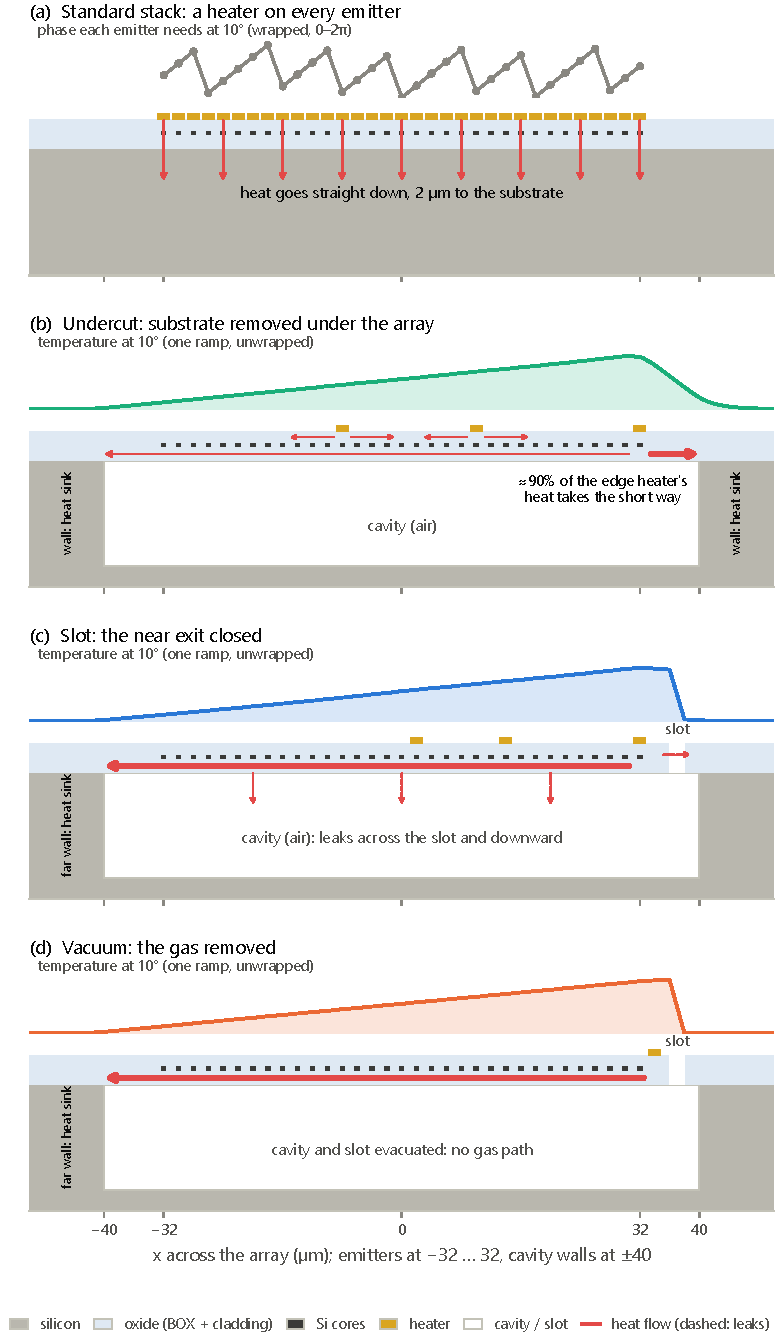
\includegraphics[height=0.62\textheight,width=\linewidth,keepaspectratio]{fig01_stacks}
  \caption{The four structures (cross-sections; heater and core thickness exaggerated), each with the phase
  profile it makes at \ang{10}. (a)~\stack{Standard}: heat flows straight into the substrate, so each emitter needs
  its own heater with a wrapped phase. (b)~\stack{Undercut}: heat spreads sideways to both cavity walls, but the
  edge heater loses most of its heat to the nearby wall. (c)~\stack{Slot}: the slot closes that short path, so the
  heat crosses the array and the temperature falls as a ramp; air still conducts some heat across the slot and into
  the cavity. (d)~\stack{Vacuum}: with no gas, the far wall is the only heat sink.}
  \label{fig:stacks}
\end{figure}

\subsection{Finite-element models}

Three two-dimensional models, built in COMSOL Multiphysics~6.3~\cite{comsol}, supply every physical input
(\cref{tab:models}). Each exports tables that the Python analysis reads directly. Meshes are free triangular, with elements of
\qtyrange{25}{35}{\nano\metre} in the cores and heater and \qtyrange{130}{250}{\nano\metre} in the oxide; their
adequacy is checked in \cref{sec:comsolchecks}.

\begin{table}[htbp]
  \centering
  \caption{The three finite-element models and their studies.}
  \label{tab:models}
  \small
  \begin{tabularx}{\linewidth}{@{}P{0.13\linewidth}P{0.4\linewidth}L@{}}
    \toprule
    Model & Studies & Outputs used \\
    \midrule
    Waveguide & mode analysis of one strip, swept in temperature and wavelength; even and odd supermodes of a
        pair, swept in spacing & $\neff$, $\dndT$, element pattern, group index; coupling length \\
    Thermal & stationary heat transfer with one heater swept across the array, for each structure; coupled
        heat-and-mode solve; step responses; temperature-dependent conductivity with two heaters & kernels
        $R(x;\xh)$; check of \cref{eq:phaseT}; transients; limits of linearity and superposition \\
    Grating & frequency-domain side view of one grating with ports and absorbing layers & emission angle and its
        rates with period, wavelength and temperature; leakage length \\
    \bottomrule
  \end{tabularx}
\end{table}

\subsubsection{Waveguide model}
\label{sec:modelA}

A mode solve of one core in a \qty{4}{\micro\metre} silica box ($n_\mathrm{Si}=3.476$, $n_\mathrm{SiO_2}=1.444$,
thermo-optic coefficients \qty{1.86e-4}{} and \qty{0.95e-5}{\per\kelvin}) gives $\neff=\num{2.44546}$. A uniform
temperature sweep over \qty{100}{\kelvin} gives
\begin{equation}
  \frac{\dd\neff}{\dd T} \;=\; \qty{2.009e-4}{\per\kelvin},
\end{equation}
linear to \num{3.5e-6} and \num{1.08} times the bulk value, because the mode is concentrated in the core
(\cref{fig:mode}). The element pattern is taken as the Fourier transform of the mode's $E_x$ summed over height; it
is \num{0.90} at \ang{20} and \num{0.87} at \ang{22.8}, and changes by less than \qty{1}{\percent} over
\qty{100}{\kelvin}. A wavelength sweep gives the group index, $n_g=4.18$.

The same model, reduced to a half-model with a perfect electric or magnetic conductor on the mirror plane, gives the
even and odd supermodes of two waveguides. Solving both on one mesh cancels the discretisation error in their
index difference $\Delta n$, which falls exponentially with spacing. The coupling length $L_c=\lambda/(2\Delta n)$
is \qty{2.2}{\metre} at \qty{2}{\micro\metre} pitch, and under \qty{1}{\percent} of the power transfers over
\qty{2}{\milli\metre} for any pitch above \qty{1.5}{\micro\metre}. Optical coupling is therefore
neglected.

\begin{figure}[htbp]
  \centering
  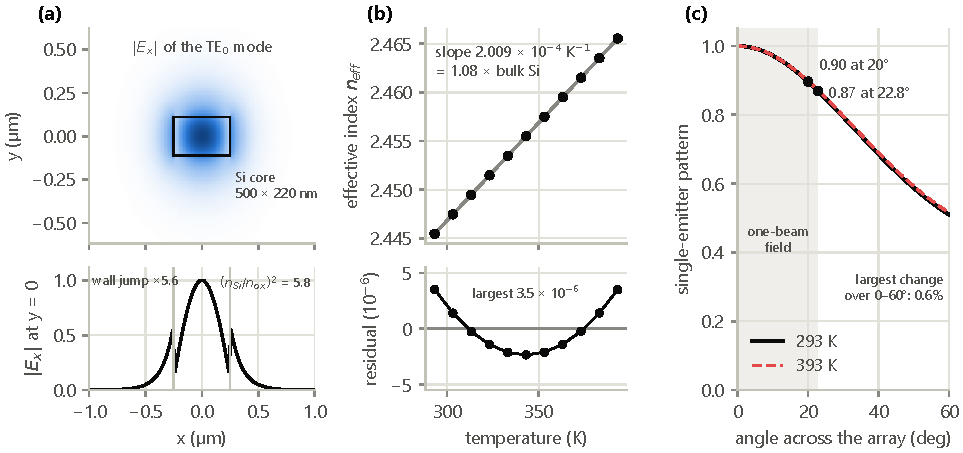
\includegraphics[width=\linewidth]{rep_mode}
  \caption{Waveguide model. (a)~$|E_x|$ of the TE mode, with a cut through the core centre; the field jumps at the
  side walls as continuity of the normal displacement requires. (b)~Effective index against temperature with its
  linear fit. (c)~Element pattern at \qty{293}{\kelvin} and \qty{393}{\kelvin}.}
  \label{fig:mode}
\end{figure}

\subsubsection{Thermal model}
\label{sec:modelC}\label{sec:modelF}

One cross-section model provides all thermal results. It contains a \qty{300}{\micro\metre}-wide,
\qty{100}{\micro\metre}-deep silicon substrate, the buried oxide, \num{33} silicon cores, the cladding and a TiN
heater that can be placed anywhere, dissipating \qty{1}{\watt\per\metre}. The substrate bottom is held at ambient
and all other boundaries are insulated; convection from the top surface would remove under \qty{1}{\percent} of
the heat. Conductivities are \qty{148}{} (Si), \qty{1.38}{} (SiO$_2$), \qty{25}{} (TiN) and
\qty{0.026}{\watt\per\metre\per\kelvin} (air). Parameters switch the structure: a cavity region becomes silicon
(\stack{standard}) or air (\stack{undercut}); a slot region through the membrane becomes oxide or air
(\stack{slot}); the gas conductivity becomes \qty{e-4}{\watt\per\metre\per\kelvin} (\stack{vacuum}; this value also
bounds black-body radiation across the cavity, $4\sigma T^3D\approx\qty{0.9e-4}{\watt\per\metre\per\kelvin}$). Four
studies were run:

\begin{enumerate}
  \item \emph{Kernels.} The temperature rise along the line through the cores, for heater positions swept in
        \qty{1}{} or \qty{2}{\micro\metre} steps: one solve for the \stack{standard} stack, whose kernel depends only
        on $x-\xh$; $\xh=0$ to \qty{40}{\micro\metre} for the \stack{undercut} (mirrored for negative positions);
        $-32$ to \qty{34}{\micro\metre} for the \stack{slot} and \stack{vacuum}, which have no mirror symmetry.
        Six further solves test the stack (\cref{sec:comsolchecks}).
  \item \emph{Coupled heat and mode.} A mode solve inside the temperature field of a heater 0, 2 and
        \qty{4}{\micro\metre} from a core, to test \cref{eq:phaseT} in a non-uniform field.
  \item \emph{Step responses.} The time-dependent response to switching a heater on, at all \num{33} cores, for
        each structure, to \qty{32}{\milli\second}.
  \item \emph{Nonlinearity.} Conductivities made temperature-dependent ($k_\mathrm{Si}\propto T^{-1.3}$,
        $k_\mathrm{SiO_2}\propto1+\qty{8e-4}{\per\kelvin}\,\Delta T$), with heater powers raised until the core is
        about \qty{185}{\kelvin} above ambient, and a second heater \qty{6}{\micro\metre} away for the superposition
        test of \cref{sec:superposition}.
\end{enumerate}

\subsubsection{Grating model}
\label{sec:modelE}

A side view of one grating gives the behaviour along the waveguides. Because the strip is three-dimensional, the
two-dimensional model uses an equivalent core of index \num{3.0604} that reproduces the strip's $\neff$ and
$\dndT$ exactly; emission angles and their rates with period and temperature therefore carry over to the real
waveguide. The rate with wavelength is corrected using the strip's group index, and the emission strength is
approximate. The model is excited through a port and terminated by absorbing layers; \num{18} runs vary period,
wavelength and temperature (results in \cref{sec:gratingaxis}).

% =====================================================================================
\section{Array analysis}
\label{sec:methods}
% =====================================================================================

The array-level questions (which heaters, at what powers, with what beam) are answered in Python in five steps
(\cref{fig:pipeline}).

\begin{figure}[htbp]
  \centering
  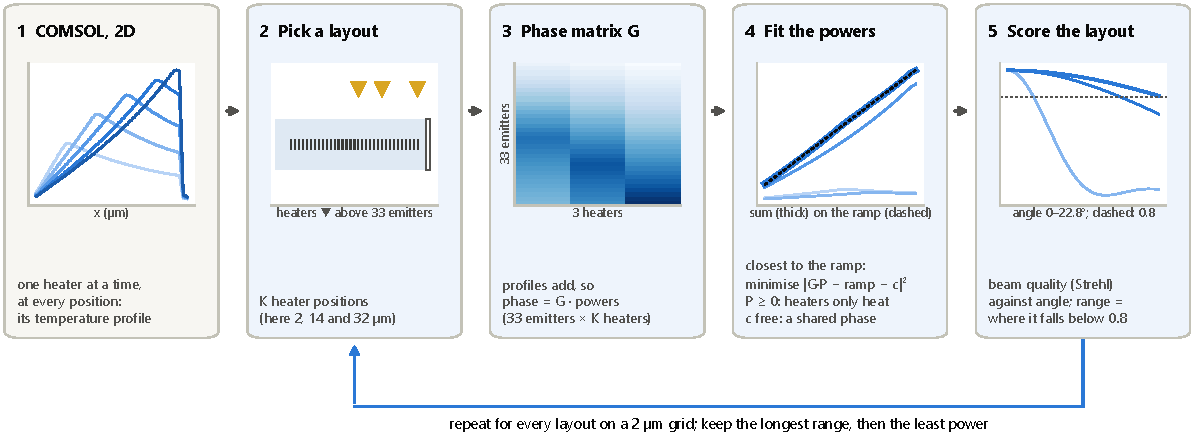
\includegraphics[width=\linewidth]{fig13_pipeline}
  \caption{The analysis. (1)~COMSOL gives the temperature profile of one heater at every position. (2)~A heater
  layout is chosen. (3)~The profiles of its heaters, scaled by $\gamma$, form the phase matrix $G$. (4)~The powers
  are fitted to a target phase profile by non-negative least squares with a free offset. (5)~The layout is scored
  by the Strehl ratio against steering angle; its range ends where this falls below \num{0.8}. Steps 2--5 repeat
  over a grid of layouts. The thumbnails are the slot design's own data.}
  \label{fig:pipeline}
\end{figure}

\subsection{Phase matrix}

$G$ (\cref{eq:G}) is assembled by evaluating the kernel at the \num{33} emitter positions. Kernel columns are
interpolated linearly in heater position; predicting a column from its neighbours \qty{2}{\micro\metre} either
side, twice the largest gap used, reproduces it to within \qty{1}{\percent} of the peak. By superposition
(\cref{sec:superposition}), a heater of width $2m$~\unit{\micro\metre} equals $m$ adjacent \qty{2}{\micro\metre}
heaters at equal power, so wide heaters need no new simulation.

\subsection{Beam quality}
\label{sec:metrics}

The far field is \cref{eq:farfield} evaluated on a fine grid in $\sin\theta$. The figure of merit is the Strehl
ratio, the intensity in the intended direction $u_0=\sin\theta_0$ relative to a perfect ramp aimed there:
\begin{equation}
  S(u_0) \;=\; \Bigl|\frac{1}{N}\sum_{n} \ee^{\,\ii(\phi_n - k_0 x_n u_0)}\Bigr|^{2}.
  \label{eq:strehl}
\end{equation}
The element pattern cancels, and $S$ depends only on the residual phase error. For a small rms residual $\sigma$,
$S\approx\ee^{-\sigma^2}$~\cite{ruze1966}. A beam is accepted when $S\ge0.8$, the usual criterion for a
diffraction-limited beam, which allows $\sigma\approx\qty{0.47}{\rad}$.

\subsection{Heater powers}
\label{sec:fit}

For a target profile $\bm\phi^{\,\mathrm t}$ (a ramp, a parabola or both) the powers and offset minimise the phase
error,
\begin{equation}
  \min_{\bm P\ge 0,\;c}\;\bigl\lVert\, G\bm P - \bm\phi^{\,\mathrm t} - c\,\bm 1 \,\bigr\rVert^{2},
  \label{eq:nnls}
\end{equation}
a non-negative least-squares problem solved with SciPy~\cite{scipy2020}; the constraint
$\bm P\ge0$ expresses that heaters cannot cool. The problem is homogeneous: scaling the target scales the optimal
powers and the residual equally. One fit to a unit ramp therefore gives the powers at every angle,
$\bm P(\theta)\propto\sin\theta$, and $S$ falls monotonically with angle, so each layout has a well-defined
\emph{range}, the largest angle with $S\ge0.8$. Power is quoted per degree, as the power at \ang{1}. The two
steering directions are fitted separately.

\subsection{Heater placement}
\label{sec:placement}

Layouts are ranked by range and then by power. For up to three heaters the search is exhaustive on a
\qty{1}{} or \qty{2}{\micro\metre} grid; for more heaters, a pattern search refines random starts. Symmetric
structures (\stack{standard}, \stack{undercut}) are ranked by their total span over both directions; the
one-sided structures (\stack{slot}, \stack{vacuum}) steer towards $+\theta$ only.

\subsection{Conventional benchmark}
\label{sec:conventional}

The reference is an ideal array of isolated heaters, one per emitter, each supplying its phase modulo $2\pi$:
\begin{equation}
  P_\mathrm{conv}(\theta) \;=\; \frac{\Ppi}{\pi}\,\min_{c}\,\sum_{n}\bigl[(n\,\Delta\phi + c)\bmod 2\pi\bigr].
  \label{eq:conv}
\end{equation}
Above about \ang{1.4} the wrapped phases fill $0$--$2\pi$ evenly and $P_\mathrm{conv}\approx0.9\,N\,\Ppi$,
independent of angle. The benchmark ignores crosstalk, calibration power and the fan-in, so it favours the
conventional design. When a published $\Ppi$ is used, the result is our estimate for an array that has not been
built, and is marked as such.

\subsection{Settling time}
\label{sec:settlemethod}

With the step responses $s_{nk}(t)$ of the thermal model, a step in drive from zero gives
$\phi_n(t)=\gamma\sum_k s_{nk}(t)P_k$. The settling time is the time after which $S\ge0.8$ towards the target is
maintained.

% =====================================================================================
\section{Verification}
\label{sec:verification}
% =====================================================================================

Verification asks whether the equations were solved correctly; validation asks whether they are the right
equations. This section covers verification. Validation is possible only indirectly, by
comparison with published devices (\cref{sec:fidelity}), since nothing was fabricated.

\subsection{Finite-element models}
\label{sec:comsolchecks}

\Cref{tab:checks} lists the checks. Each quantity used in the analysis was recomputed on finer meshes and larger
domains; every thermal run was tested for energy balance (heat leaving through the substrate equals the
\qty{1}{\watt\per\metre} supplied); the grating model was tested for power balance and against the grating
equation; and quantities computed by two different studies were compared.

\begin{table}[htbp]
  \centering
  \caption{Verification checks on the finite-element models. ``Result'' is the change in, or value of, the quantity
  used by the analysis.}
  \label{tab:checks}
  \footnotesize
  \begin{tabularx}{\linewidth}{@{}P{0.27\linewidth}P{0.2\linewidth}P{0.22\linewidth}L@{}}
    \toprule
    Check & Quantity & Result & Criterion \\
    \midrule
    \multicolumn{4}{@{}l}{\emph{Waveguide model}} \\
    mesh refined ($35/150\to18/70$\,nm) & $\neff$ & \num{4.5e-5} & $<\num{1e-4}$ \\
    box widened \qtyrange{4}{8}{\micro\metre} & $\neff$ & \num{2e-6} & $<\num{1e-4}$ \\
    linearity over \qty{100}{\kelvin} & deviation from fit & \num{3.5e-6} & $\ll$ total change \num{2.0e-2} \\
    decay of supermode splitting & slope of $\ln\Delta n$ & \qty{8.3}{\per\micro\metre} & mode tail,
        $\approx\qty{8}{\per\micro\metre}$ \\
    \addlinespace
    \multicolumn{4}{@{}l}{\emph{Thermal model}} \\
    energy balance, every stationary run & heat out / heat in & worst \qty{0.05}{\percent} off & within
        \qty{1}{\percent} \\
    finer oxide mesh (\qtyrange{250}{125}{\nano\metre}) & core rise & $<\qty{0.1}{\percent}$ & $<\qty{1}{\percent}$ \\
    domain width $\pm150\to\pm\qty{300}{\micro\metre}$ & core rise & $-\qty{0.04}{\percent}$ & $<\qty{1}{\percent}$ \\
    substrate depth \qtyrange{100}{200}{\micro\metre} & core rise & $+\qty{1.2}{\percent}$, uniform to \num{e-4} &
        common offset only \\
    oxide in place of Si cores & core rise & $+\qty{3}{\percent}$ at peak & informative \\
    buried oxide \qtyrange{2}{3}{\micro\metre} & core rise & $+\qty{26}{\percent}$ & design parameter \\
    mode solved in the heated field & solved / predicted $\Delta\neff$ & \num{0.999}, \num{0.997}, \num{1.000} &
        within \qty{3}{\percent} \\
    step responses at late time & against stationary kernels & within \qty{0.01}{\percent} & within
        \qty{1}{\percent} \\
    step-response overshoot & excess over final value & $\le\qty{0.14}{\percent}$ & $<\qty{0.5}{\percent}$ \\
    \stack{vacuum} ramp & rms deviation from a line & \qty{0.016}{\percent} & $<\qty{1}{\percent}$ \\
    \stack{vacuum} power & against conduction limit & \num{0.532} vs \qty{0.506}{\mWdeg} & within
        \qty{5}{\percent}, nothing fitted \\
    \addlinespace
    \multicolumn{4}{@{}l}{\emph{Grating model}} \\
    power balance, \num{18} runs & $R+T+\text{up}+\text{down}$ & \numrange{1.005}{1.011} & within
        \qty{3}{\percent} \\
    grating equation, \num{18} runs & emission angle & within \ang{0.03} & nothing fitted \\
    leakage against transmission & $T$ over \qty{34.5}{\micro\metre} & \qty{73}{\percent} predicted,
        \qty{71}{\percent} found & consistent \\
    \bottomrule
  \end{tabularx}
\end{table}

Mesh and domain width change the \stack{standard} kernel by less than \qty{0.1}{\percent}. A deeper substrate adds \qty{1.2}{\percent} of the peak to every core equally, which
is a common phase and does not affect steering. The buried-oxide thickness changes the kernel substantially and is
a design parameter, fixed at \qty{2}{\micro\metre}.

Mesh convergence was tested with two or three meshes
per quantity and is reported as the observed change, not as a formal grid-convergence index; the changes are two
orders of magnitude below the effects reported.
\subsection{Python model}
\label{sec:pipelinechecks}

Before any result was computed, the Python model was run against \num{54} checks with known answers; all pass
(\cref{tab:pipelinechecks}). They confirm that the constants and kernels are read
correctly from the COMSOL data; that the far field reproduces the analytic beam width $0.886\,\lambda/(Nd)$, the
\qty{13.26}{\decibel} first side lobe, the steering law \cref{eq:steer} and the two equal beams at
$\Delta\phi=\pi$; that the mean Strehl ratio for random errors follows the finite-$N$ Ruze formula (\cref{eq:ruze});
and that the fit satisfies its optimality conditions and reproduces the exact conventional power for isolated
heaters.

\begin{table}[htbp]
  \centering
  \caption{Checks on the Python model; all \num{54} pass.}
  \label{tab:pipelinechecks}
  \small
  \begin{tabularx}{\linewidth}{@{}P{0.24\linewidth}Lc@{}}
    \toprule
    Group & Compared with & Checks \\
    \midrule
    Constants & $\dndT$ refitted from the waveguide model; $\gamma$ & 2 \\
    Kernels & peak values, $\Ppi$, ratios at 2--\qty{32}{\micro\metre}, symmetry, interpolation & 15 \\
    Temperature to phase & coupled mode solve & 3 \\
    Phase matrix & emitter positions; mirror rule & 5 \\
    Element pattern & \num{0.90} at \ang{20}, \num{0.87} at \ang{22.8} & 2 \\
    Far field & beam angle, width, side and grating lobes, ramps, $\Delta\phi=\pi$ & 16 \\
    Statistics & mean Strehl against the Ruze relation & 3 \\
    Fit & scaling, optimality of the residual & 4 \\
    Conventional benchmark & known powers; diagonal $G$ & 4 \\
    \bottomrule
  \end{tabularx}
\end{table}
\subsection{Assumptions not verified}
\label{sec:notverified}

Three assumptions are not tested by any simulation and are listed as limitations (\cref{sec:limitations}): heat
flow is two-dimensional (no heater or cavity ends, and no heat conducted along the waveguides to the gratings);
emitters are identical and independent in the far-field model; and the pressure needed for vacuum operation relies on
a simple kinetic model of gas conduction.

% =====================================================================================
\section{Results: steering}
\label{sec:steering}
% =====================================================================================

The four structures are compared using three measures: the steering range at $S\ge0.8$, the power per degree, and
the settling time.

\subsection{Thermal kernels}
\label{sec:kernels}

\Cref{fig:kernels}(a) shows the temperature produced by one centred heater. On the \stack{standard} stack the heat
sink is \qty{2}{\micro\metre} below the cores. The core under the heater rises by \qty{0.196}{\KmW}
($\Ppi=\qty{19.7}{\milli\watt}$), and the profile has a half-width of \qty{3.3}{\micro\metre}: the cores 2, 4 and
\qty{8}{\micro\metre} away receive \num{0.75}, \num{0.41} and \num{0.12} of the peak, so $\Lth/d\approx1.7$. On the
\stack{undercut} membrane, heat can leave only sideways to the cavity walls and weakly through the air below. The
same heater raises its core by \qty{2.85}{\KmW} ($\Ppi=\qty{1.35}{\milli\watt}$), and the half-width is
\qty{20.6}{\micro\metre}: the cores 8, 16 and \qty{32}{\micro\metre} away receive \num{0.81}, \num{0.61} and \num{0.23}
of the peak, so $\Lth/d\approx10$ and one heater reaches the whole array. Both single-heater values agree with
measured devices of each kind (\cref{sec:fidelity}).

\begin{figure}[htbp]
  \centering
  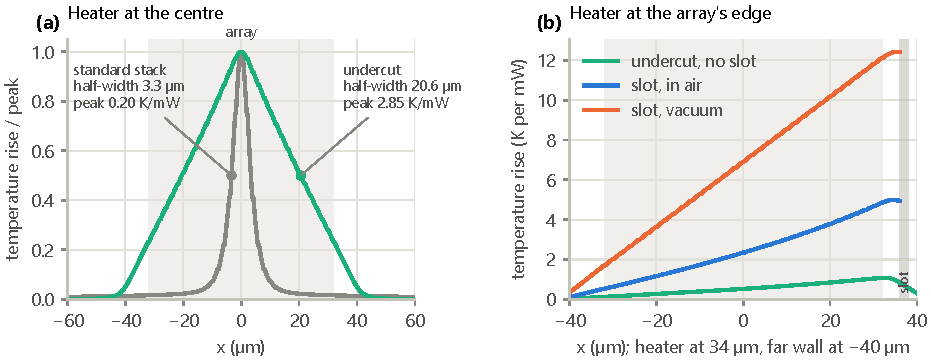
\includegraphics[width=\linewidth]{fig02_kernels}
  \caption{Temperature profile of one \qty{1}{\milli\metre} heater. (a)~Heater at the centre: half-width
  \qty{3.3}{\micro\metre} on the \stack{standard} stack and \qty{20.6}{\micro\metre} on the \stack{undercut}, which
  is \num{14} times hotter per milliwatt. (b)~Heater at the edge (\qty{34}{\micro\metre}): without a slot, little
  heat reaches the array; with a slot in air the profile is nearly linear; in vacuum it is linear and \num{2.5} times
  steeper.}
  \label{fig:kernels}
\end{figure}

\subsection{Standard stack}
\label{sec:standardfails}

On the \stack{standard} stack few heaters cannot steer. The best layout of eight heaters reaches a total span of
only \ang{3.4}, at \qty{60}{\mWdeg}: eight profiles \qty{3.3}{\micro\metre} wide leave most of the
\qty{64}{\micro\metre} aperture unheated. Steering one way across the full field requires \num{24} heaters. The
heated-section pitch matters as expected: \num{16} evenly spaced heaters steer \ang{18.6} at a
pitch of \qty{1.5}{\micro\metre} ($\Lth/d=2.2$) but only \ang{1.5} at \qty{4}{\micro\metre} ($\Lth/d=0.84$). With a
heater on every emitter and wrapped phases, the \stack{standard} stack needs \qtyrange{468}{580}{\milli\watt} between
\ang{1} and \ang{10}.
\subsection{Undercut membrane}
\label{sec:undercut}

On the \stack{undercut} membrane one edge heater already steers \ang{4.4}. Three heaters steer \ang{\pm 12} and four
reach \ang{\pm 16.0} at \qty{4.94}{\mWdeg}. With the outer pair placed just beyond the last emitters, four heaters
at $-32.75$, $-6.7$, $9.4$ and \qty{32.6}{\micro\metre} steer the full \ang{\pm 22.8} at \qty{5.24}{\mWdeg}.

The undercut design is inefficient. At \ang{10} it needs \qty{49}{\milli\watt}, while an ideal array of isolated
heaters with the same membrane's $\Ppi$ needs \qty{40}{\milli\watt}; the membrane is better only below about
\ang{8}. The reason is visible in \cref{fig:kernels}(b). An edge heater is \qty{8}{\micro\metre} from one cavity wall
and \qty{72}{\micro\metre} from the other. Each side conducts $\kt\,T_\mathrm{h}/\ell$ for a heater temperature $T_\mathrm{h}$, so the heat divides in inverse
proportion to the distances, and about \qty{90}{\percent} flows into the near wall without contributing to the ramp.

\subsection{Slot and vacuum}
\label{sec:slot}

If the membrane is cut just beyond the edge heater, the near wall can no longer be reached. All the heat must then
cross the array to the far wall, and with no losses in between the temperature is a straight line
(\cref{sec:superposition}).

\paragraph{Conduction limit.} The required power follows directly. All the heater power per unit length crosses the
membrane, $P/\Lh=\kt\,\dd T/\dd x$, and the steering angle sets the phase gradient,
$\Delta\phi/d=\gamma\Lh\,\dd T/\dd x$. Eliminating the gradient,
\begin{equation}
  P \;=\; \frac{\kt\,\Delta\phi}{\gamma\,d} \;=\; \qty{0.506}{\milli\watt}\ \text{per degree}
  \qquad(\kt=\qty{5.82e-6}{\watt\per\kelvin}).
  \label{eq:limit}
\end{equation}
This is independent of the number of emitters and of the heater length, because the same heat flux passes every
emitter. What grows with array size is the temperature at the hot end, proportional to $N$, and the settling time,
proportional to the square of the span.

\paragraph{Vacuum.} With no gas in the cavity or slot, one heater at \qty{34}{\micro\metre} produces a ramp straight
to \qty{0.016}{\percent} rms and steers the full \ang{22.8} at \qty{0.532}{\mWdeg} (\qty{5.3}{\milli\watt} at
\ang{10}), within \qty{5}{\percent} of \cref{eq:limit} with nothing fitted. Most of the difference is due to the
silicon cores, which add to the membrane's $\kt$, and the small residual gas conductivity. Additional heaters do not
reduce the power.

\paragraph{Air.} In air the single heater steers only \ang{4.0}, at \qty{1.30}{\mWdeg}. Two losses remain. Heat
escapes downward through the cavity air along the whole membrane, which curves the ramp (rms deviation
\qty{2.6}{\percent} of its rise, about \qty{1}{\rad} at \ang{10}). Air also conducts across the slot: its conductance
$k_\mathrm{air}t/w$ equals that of about \qty{106}{\micro\metre} of oxide membrane, comparable with the
\qty{74}{\micro\metre} path across the array.

Interior heaters correct the curvature (\cref{fig:placement}). With the edge heater at \qty{32}{\micro\metre}, a
second heater at \qty{5}{\micro\metre} extends the range to \ang{17.2}, and a third, with heaters at 2, 14 and
\qty{32}{\micro\metre}, reaches the full \ang{22.8} at
\begin{equation}
  \qty{1.38}{\mWdeg}, \quad\text{that is, } \qty{13.8}{\milli\watt}\ \text{at}\ \ang{10}.
\end{equation}
Of the \num{1891} three-heater layouts on a \qty{1}{\micro\metre} grid, \num{263} reach the full range, so the design
is not sensitive to exact positions. A \qty{4}{\micro\metre} slot reaching the wall reduces the power by a further
\qty{12}{\percent}, to \qty{1.22}{\mWdeg}.

\begin{figure}[htbp]
  \centering
  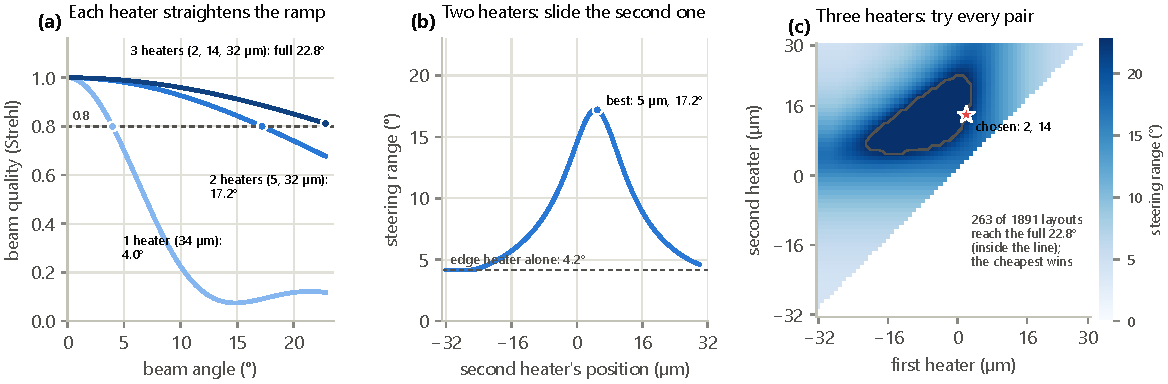
\includegraphics[width=\linewidth]{fig16_placement}
  \caption{Heater placement on the slot membrane. (a)~Strehl ratio against angle for the best layout of one, two and
  three heaters: ranges \ang{4.0}, \ang{17.2} and \ang{22.8}. (b)~Two heaters: range against the position of the
  second, edge heater at \qty{32}{\micro\metre}. (c)~Three heaters: range for every pair of interior positions;
  outlined layouts reach the full range.}
  \label{fig:placement}
\end{figure}

\Cref{fig:ramp} shows this design. The edge heater carries \qty{83}{\percent} of the power and produces the ramp;
the two interior heaters correct the curvature caused by the air loss. The resulting profile follows the ideal ramp
with $S=0.96$ at \ang{10}. Other angles require only scaling the three powers by $\sin\theta/\sin\ang{10}$.

\begin{figure}[htbp]
  \centering
  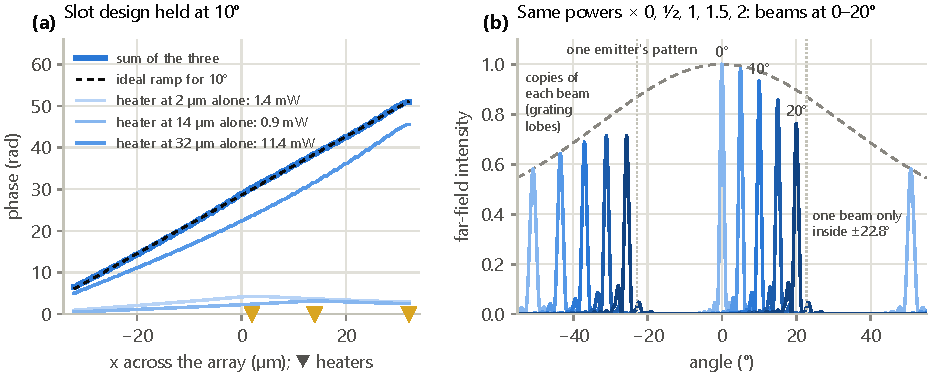
\includegraphics[width=\linewidth]{fig03_ramp_and_beams}
  \caption{The slot design (heaters at 2, 14 and \qty{32}{\micro\metre}). (a)~Phase at \ang{10}: each heater's
  contribution, their sum, and the ideal ramp. (b)~Far field at \ang{0}--\ang{20} in \ang{5} steps, powers scaled by
  $\sin\theta/\sin\ang{10}$. The dashed curve is the element pattern; each beam has a grating lobe at
  $\sin\theta-\lambda/d$.}
  \label{fig:ramp}
\end{figure}

\begin{table}[htbp]
  \centering
  \caption{Summary of the designs (simulated; $N=33$, $d=\qty{2}{\micro\metre}$). Range at $S\ge0.8$; ``$\pm$''
  denotes two-sided, otherwise one way. Settling is for a step from \ang{0} to \ang{10}.}
  \label{tab:designs}
  \footnotesize
  \setlength{\tabcolsep}{4.5pt}
  \begin{tabular}{@{}lcllccc@{}}
    \toprule
    Design & Wires & Heaters (\unit{\micro\metre}) & Range & \unit{\mWdeg} & $P_{10^\circ}$ (\unit{\milli\watt}) &
    Settling (\unit{\milli\second}) \\
    \midrule
    \stack{Standard}, isolated, wrapped & 33 & every emitter & \ang{\pm 22.8} & --- & 580 & $\approx0.02$\textsuperscript{a} \\
    \stack{Undercut} & 3 & $-8$, 10, 32 & \ang{15.9} & 4.93 & 49 & 2.0 \\
    \stack{Undercut}, heaters to the walls & 4 & $\pm32.7$, $-6.7$, 9.4 & \ang{\pm 22.8} & 5.24 & 52 & --- \\
    \stack{Slot} (air) & 3 & 2, 14, 32 & \ang{22.8} & 1.38 & 13.8 & 3.5 \\
    \stack{Vacuum} & 1 & 34 & \ang{22.8} & 0.53 & 5.3 & 8.8 \\
    \bottomrule
  \end{tabular}

  \vspace{2pt}
  \begin{minipage}{0.96\linewidth}\footnotesize
  \textsuperscript{a}\,Estimated from one heater's step response reaching \qty{92}{\percent}. Settling times of the
  membranes were computed for the nearest layouts on the \qty{4}{\micro\metre} grid of the transient runs
  (\stack{undercut} $-12$, 8, 32; \stack{slot} 0, 12, \qty{32}{\micro\metre}), whose powers differ by under
  \qty{1}{\percent}.
  \end{minipage}
\end{table}

\subsection{Comparison with a conventional array}
\label{sec:power}

\Cref{fig:power} compares the hold power with that of ideal conventional arrays. A wrapped array holds any angle
above about \ang{1.4} for roughly $0.9\,N\,\Ppi$, since no element needs more than $2\pi$. Our power grows with
$\sin\theta$, since the ramp is built in full. Per radian of phase the membrane is the more efficient actuator: the
\stack{vacuum} design uses \qty{7}{\micro\watt} per radian per emitter and the \stack{slot} design
\qty{18}{\micro\watt}, against \qty{16}{\micro\watt} for the best published folded phase shifter~\cite{lu2015} and
\qty{156}{\micro\watt} for the best single-pass suspended one~\cite{fang2011}. At \ang{10}, however, our ramp sums to
\qty{743}{\rad} over the array, while a wrapped array needs about \qty{92}{\rad}. As a result:
\begin{itemize}
  \item against a conventional \stack{standard}-stack array, the \stack{slot} and \stack{vacuum} designs need
        \num{42} and \num{110} times less power at \ang{10};
  \item against \num{33} single-pass suspended heaters (\qty{0.49}{\milli\watt}~\cite{fang2011}), the \stack{slot}
        design is lower below \ang{10.3} and equal at \ang{10};
  \item against \num{33} folded record shifters (\qty{50}{\micro\watt}~\cite{lu2015}), the \stack{vacuum} design is
        lower only below \ang{2.8} and \num{3.6} times higher at \ang{10}.
\end{itemize}
The last two cases are estimates for arrays that have not been built; they assume no crosstalk or calibration
power, and the record device is a \qty{6}{\milli\metre} folded Michelson switch.

\begin{figure}[htbp]
  \centering
  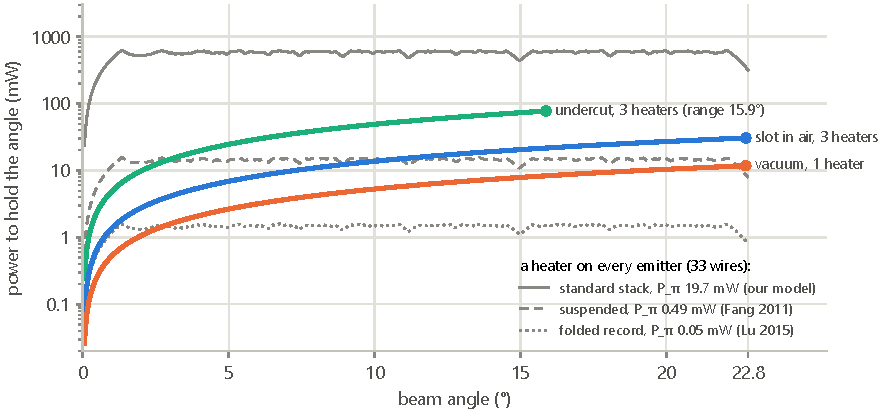
\includegraphics[width=0.86\linewidth]{fig04_power_vs_angle}
  \caption{Power to hold each angle, $N=33$. Grey: ideal conventional arrays (one isolated heater per emitter,
  wrapped phases) at three phase-shifter efficiencies. Colours: this work, one to three wires.}
  \label{fig:power}
\end{figure}

The slot and vacuum reduce power but not temperature. At \ang{10} the hottest core is \qtyrange{62}{64}{\kelvin}
above ambient for \qty{1}{\milli\metre} heaters in every design, because the required phase fixes it
($\Delta T=\phi/(\gamma\Lh)$); only a longer heater lowers it. A wrapped array never exceeds \qty{7.7}{\kelvin}.

\subsection{Speed}
\label{sec:speed}

A heater on the \stack{standard} stack warms its core to \qty{90}{\percent} in \qty{21}{\micro\second}; on the
\stack{undercut} membrane this takes \qty{1.63}{\milli\second}, \num{77} times longer for \num{14.5} times less power
(\cref{fig:transients}a). For a beam step from \ang{0} to \ang{10}, the Strehl ratio reaches and holds \num{0.8} after
\qty{2.0}{} (\stack{undercut}), \qty{3.5}{} (\stack{slot}) and \qty{8.8}{\milli\second} (\stack{vacuum}), that is,
bandwidths of roughly \num{190}, \num{110} and \qty{50}{\hertz} (\cref{fig:transients}b).

Two effects make these times long. First, a profile of spatial period $\Lambda$ relaxes at a rate
$\alpha(2\pi/\Lambda)^2+h/(\rho c\,t)$, so the ramp, the broadest profile, is the slowest; removing heat paths to save
power also removes paths by which the membrane settles, which is why vacuum is slower than air. Second, an
unwrapped \ang{10} ramp spans \qty{45}{\rad}, so the membrane must reach about \qty{99}{\percent} of its final state to
leave less than \qty{0.47}{\rad} of error, whereas a wrapped element needs about \qty{92}{\percent}. Small steps are
faster: a \ang{1} correction settles in \qty{0.36}{}, \qty{0.80}{} and \qty{2.4}{\milli\second}.

\begin{figure}[htbp]
  \centering
  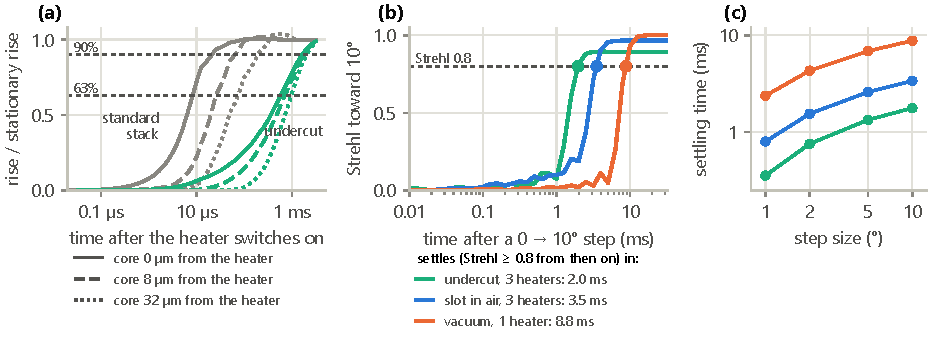
\includegraphics[width=\linewidth]{rep_transients}
  \caption{Speed with step drives. (a)~Single-heater step responses, \stack{standard} and \stack{undercut}.
  (b)~Strehl ratio towards \ang{10} after a step from \ang{0}. (c)~Settling time against step size.}
  \label{fig:transients}
\end{figure}

\subsection{Shaped drives (pre-emphasis)}
\label{sec:preemphasis}

A step drive is slow because each heater supplies only its final power from the start. Because conduction is
linear (\cref{sec:superposition}), the phase produced by any drive $P_k(t)$ is a sum of time-shifted step responses,
so the drive can be designed to reach the target sooner: each heater is first driven above its final power and then
brought back, and heaters whose heat arrives too strongly at some emitters are briefly turned down.

\paragraph{Method.} Each heater's drive is piecewise constant (30 intervals before the target time $T$, 15 after),
non-negative, and must end on the step's final powers, so every drive holds the same beam. The chip's total power
may not exceed $m$ times its hold power at \ang{10}. From $T$ onwards the rms phase error is required to stay below
$\sigma^*=\sqrt{2(1-\sqrt{0.8})}=\qty{0.46}{\rad}$, which guarantees $S\ge0.8$ since
$|\langle\ee^{\ii\varepsilon}\rangle|\ge1-\sigma^2/2$. This rms limit is a convex constraint, imposed with cutting
planes, so for each $T$ the drive is a linear program; bisection on $T$ gives the shortest settling time, and among
the drives that achieve it the one closest to the hold drive is kept. Two checks fix the method. For a single
thermal mode the optimal overdrive settles in $\tau\ln[m/(m-1+\varepsilon)]$, which the program reproduces to
\qty{0.3}{\percent}. With $m=1$ and one heater it returns the plain step. Doubling the time grids leaves $T$
unchanged. The settling times in this subsection are evaluated on a finer time grid than in \cref{sec:speed}, which
shortens the plain-step times by \qty{2.5}{\percent}.

\paragraph{Results.} With the chip allowed three times its hold power for a moment, a step from \ang{0} to \ang{10}
settles in \qty{0.43}{\milli\second} instead of \qty{3.42}{\milli\second} for the \stack{slot} design (\num{8} times
faster), \qty{1.43}{} instead of \qty{8.54}{\milli\second} in \stack{vacuum} (\num{6} times) and \qty{0.16}{} instead of
\qty{1.94}{\milli\second} on the \stack{undercut} (\num{12} times) (\cref{fig:preemphasis}). At twice the hold power the
gains are \numrange{4}{9} times. The extra energy per step is \qtyrange{9}{13}{\micro\joule}.

The gain comes from driving the heaters independently. One overdrive waveform shared by all heaters gives only
\numrange{3}{4} times, and overheats the hottest core to \numrange{1.5}{2.3} times its final temperature; with
independent drives the hottest core stays within \qty{8}{\percent} of its final value for the \stack{slot} design.
Two heaters already give \num{7.3} times, and seventeen give \num{10.7} times, so the few-wire design keeps most of
the available gain. Small corrections gain most: a \ang{1} step from a held angle settles \numrange{10}{19} times
faster. A return to \ang{0} cannot be accelerated, since all heaters are then already off; if fast returns matter,
the rest position can be set at a small standing tilt.

\paragraph{Sensitivity.} The drive is computed from the thermal model, so it depends on the model's time scale. If
the device's heat flow is \qty{2}{\percent} slower than modelled, the \stack{slot} design's \num{8}-fold gain falls to
about \num{3}; the planned cut-back then arrives before the heat. A drive designed to work over a $\pm\qty{5}{\percent}$
range of time scales keeps a gain of \num{6.8} (\qty{0.51}{\milli\second}) for the \stack{slot} design and \num{5.6}
(\qty{1.54}{\milli\second}) in \stack{vacuum}, and \ang{1} corrections lose less than \qty{20}{\percent} of their gain for
a $\pm\qty{10}{\percent}$ error. In practice each heater's step response would be measured on the device before the
drives are computed.

\begin{figure}[htbp]
  \centering
  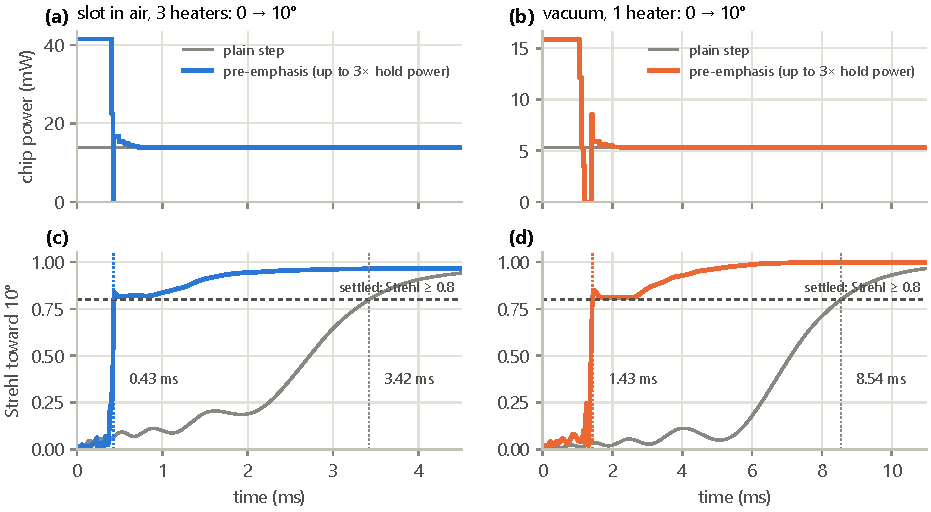
\includegraphics[width=\linewidth]{fig06_preemphasis}
  \caption{Pre-emphasis for a step from \ang{0} to \ang{10}. (a,~b)~Total chip power for the plain step and for the
  optimised drive, limited to three times the hold power, for the \stack{slot} (three heaters) and \stack{vacuum} (one
  heater) designs. (c,~d)~Strehl ratio towards \ang{10}; the settling time is where it last crosses \num{0.8}.}
  \label{fig:preemphasis}
\end{figure}

\Cref{fig:powerspeed} plots hold power against settling time. Along the design path each structure trades speed for
power. With plain steps, the product of power and settling time for a \ang{10} step is about
\qty{14}{\milli\watt\,\milli\second} for the conventional \stack{standard} array and
\qtyrange{46}{96}{\milli\watt\,\milli\second} for the membranes, against \numrange{0.5}{5} for published phase
shifters scaled to \num{33} elements. With pre-emphasis the membranes reach \qtyrange{6}{8}{\milli\watt\,\milli\second},
within \numrange{1.2}{16} times of the published devices driven with plain steps, and level with them for small
corrections.

\begin{figure}[htbp]
  \centering
  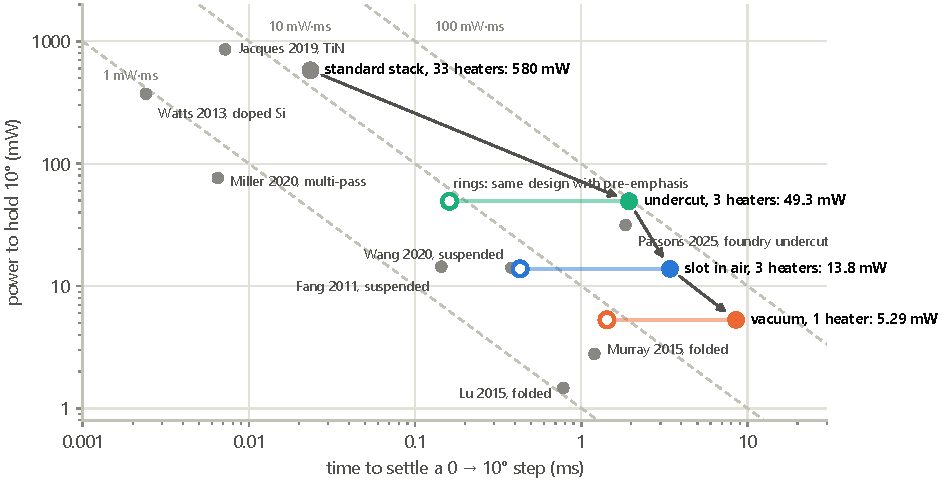
\includegraphics[width=0.9\linewidth]{fig05_power_vs_speed}
  \caption{Power to hold \ang{10} against the time to settle a step from \ang{0}. Filled circles: the four
  structures with a plain step. Rings: the same designs with pre-emphasis at up to three times the hold power. Grey:
  published single phase shifters~\cite{jacques2019,watts2013,miller2020,wang2020,fang2011,parsons2025,murray2015,lu2015}
  scaled to \num{33} isolated, wrapped heaters at their measured $\Ppi$, with the slower of their rise and fall
  times (our estimate). Dashed: constant power $\times$ time.}
  \label{fig:powerspeed}
\end{figure}

% =====================================================================================
\section{Results: patterns, errors and focusing}
\label{sec:other}
% =====================================================================================

\subsection{Usable phase patterns}
\label{sec:modes}

To find what each structure can do at best, we place a heater under every emitter, so that $G$ is $N\times N$, and
remove the free offset. The singular value decomposition $G=U\Sigma V^{\mathsf T}$ gives independent phase patterns
$\bm u_i$ with gains $s_i$ (rad/W); the power for a given amount of pattern $i$ scales as $1/s_i$. A pattern is
counted as usable if it costs at most ten times the cheapest ($s_i\ge0.1\,s_1$).

On the \stack{standard} stack at \qty{2}{\micro\metre} pitch, \num{15} of \num{32} patterns are usable, and all cost
about the same: the heaters act as independent phase shifters. On the membranes the gains fall steeply: \num{4} patterns are usable on the \stack{undercut}, \num{3} on the \stack{slot} and \num{2} in
\stack{vacuum}. For a kernel that depends only on $x-\xh$, the singular vectors approach Fourier modes of spatial
frequency $q_m\approx\pi m/(Nd)$ and the gains approach the kernel's Fourier transform. For a Gaussian kernel of
half-width $\Lth$ the gains fall as $\exp(-q^2\Lth^2/4\ln2)$, so the number of patterns above the threshold is
\begin{equation}
  M \;\approx\; \frac{\sqrt{2\ln 10}\,\sqrt{2\ln 2}}{\pi}\,\frac{N d}{\Lth}\;\approx\;0.80\,\frac{N d}{\Lth}.
  \label{eq:modecount}
\end{equation}
This predicts \num{11.8}, \num{15.8} and \num{31.6} for pitches of \num{1.5}, \num{2} and \qty{4}{\micro\metre}; the
computed counts are \num{11}, \num{15} and \num{32}.

The cheapest patterns on the membranes are their simplest steady states: a ramp (heater to sink)
and a dome (between two sinks). On the one-sided \stack{slot} and \stack{vacuum} membranes the ramp is cheapest; on
the two-walled \stack{undercut} the dome and ramp cost the same. These are exactly the two patterns used for steering
and focusing, and the third pattern already costs \numrange{4}{14} times more. Since heaters can only heat, the
\stack{vacuum} membrane cannot even form the dome: all its heater profiles rise monotonically towards the slot, so
any combination with $P_k\ge0$ is monotonic.

As a direct test, each structure was asked to split the beam into two at $\pm\theta$ with all \num{33} heaters. The
\stack{standard} stack reaches the ideal efficiency of the finite array (\numrange{0.62}{0.76} of the light in the
two beams). The membranes reach at most \num{0.46} at \ang{\pm 3} and less than \num{0.03} at \ang{\pm 5} or more,
because the required phase features ($\lambda/\sin\theta$, \qty{9}{\micro\metre} at \ang{10}) are narrower than their
\qtyrange{20}{30}{\micro\metre} spreading. The arrangement best suited to sharp patterns is therefore short spreading
($\Lth/d\lesssim2$) with a heater under every emitter, which is the conventional design.
\subsection{Fabrication errors}
\label{sec:fab}

Each waveguide carries a static phase error from width and thickness variations. We model the errors as Gaussian
with rms $\sigma$ and correlation $\exp(-\Delta x^2/2\ell^2)$ between waveguides $\Delta x$ apart; $\ell=0$ is the
independent case. Measured silicon-photonic variation has a smooth wafer-scale part (about \qty{80}{\percent} of the
width variance) and a local part uncorrelated between sites~\cite{xing2023}; the local part accumulates along a
waveguide as $\sigma^2\approx L/L_\mathrm{coh}$, with $L_\mathrm{coh}=\qty{4.17}{\milli\metre}$ for strip
waveguides~\cite{yang2015}. Three cases are compared by Monte Carlo: uncorrected, corrected by refitting the heaters
with \cref{eq:nnls}, and trimmed (error removed).

\paragraph{Independent errors.} For independent Gaussian errors the mean Strehl ratio of \cref{eq:strehl} is
\begin{equation}
  \langle S\rangle \;=\; \ee^{-\sigma^{2}} + \frac{1-\ee^{-\sigma^{2}}}{N},
  \label{eq:ruze}
\end{equation}
since the $N$ diagonal terms of $|\sum_n\ee^{\ii\varepsilon_n}|^2$ equal one and each off-diagonal term averages to
$\ee^{-\sigma^2}$~\cite{ruze1966}. After correction every design stays on this curve (\cref{fig:ruze}a): at
$\sigma=\qty{1}{\rad}$ the corrected Strehl ratio is \numrange{0.39}{0.43}, against \num{0.39} without correction. A
fit onto $K$ heater profiles plus the offset removes on average only $(K+1)/N$ of the variance of independent noise:
\qty{6}{\percent} for one heater, \qty{12}{\percent} for three.

\paragraph{Smooth errors.} Errors correlated over $\ell\gtrsim\qtyrange{16}{32}{\micro\metre}$ consist mainly of
offset, gradient and curvature, which the heaters can produce, and are corrected. At
$\ell=\qty{32}{\micro\metre}$ and $\sigma=\qty{1}{\rad}$, one heater raises $S$ from \num{0.78} to \num{0.96}, at an
extra power below \qty{0.2}{\milli\watt}.

\paragraph{Static trim.} Without trim, $S\ge0.9$ limits each waveguide's independent path to
$-L_\mathrm{coh}\ln0.9=\qty{0.44}{\milli\metre}$. A \ang{10} heated section kept below \qty{60}{\kelvin} is already
\qty{1.04}{\milli\metre} long, which alone limits an untrimmed array to $S\approx0.78$ (\cref{fig:ruze}b). The design
therefore requires a one-time static trim of each waveguide's phase beyond small angles. Trimming has been
demonstrated on ring resonators~\cite{jayatilleka2021} but, to our knowledge, not on an OPA. With trim, the
comparison with a conventional array is a one-time trim plus $K$ wires against $N$ wires plus a calibration for each
beam direction, which takes from \qty{40}{\second} to an hour per beam~\cite{lian2024}.

\begin{figure}[htbp]
  \centering
  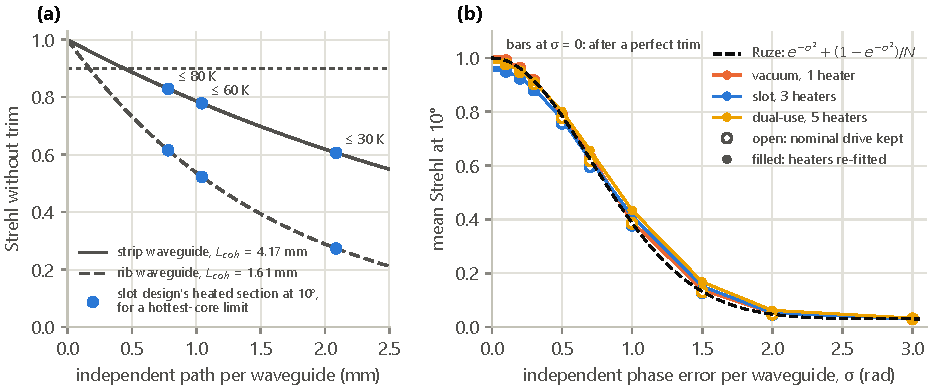
\includegraphics[width=\linewidth]{rep_ruze}
  \caption{Independent phase errors. (a)~Mean Strehl ratio at \ang{10} against rms error, uncorrected and corrected
  by the heaters, with \cref{eq:ruze}. (b)~Without trim: Strehl ratio against independent path length, with the
  heated-section length at \ang{10} for three limits on the hottest core.}
  \label{fig:ruze}
\end{figure}
\subsection{Tunable lens}
\label{sec:lens}

In vacuum the membrane temperature obeys $\kt\,T''=-q$, with $q$ the heater power per unit area. A parabola requires
$T''$ constant, which is produced by heat deposited uniformly across the array between two cold walls. For a heater
of width $W=2X$ carrying $P/\Lh$ per unit length, $q=P/(\Lh W)$ and, by symmetry, $T(0)-T(x)=qx^2/(2\kt)$ over the
heated strip: an exact parabola. The lens strength is $a=\gamma\Lh[T(0)-T(X)]$, so the power per radian is
\begin{equation}
  \frac{P}{a} \;=\; \frac{2\,\kt\,W}{\gamma\,X^{2}} \;=\; \qty{0.89}{\milli\watt\per\rad}
  \qquad (W=\qty{64}{\micro\metre},\ X=\qty{32}{\micro\metre}).
  \label{eq:lenspower}
\end{equation}
Since $\dndT>0$, heating the centre lengthens its optical path and the lens converges. A parabola needs cold walls
on both sides, so the lens uses the \stack{undercut} membrane rather than the slotted one.

\Cref{fig:lens} shows the result in a two-dimensional scalar simulation of the light above the array, with each
emitter a line source carrying the phase the heaters produce. Asked for a lens of $f=\qty{0.15}{\milli\metre}$, a single
narrow centre heater produces a tent of phase rather than a parabola, and the light spreads into a long streak with
only \num{0.22} of a perfect lens's intensity at the focus (\cref{fig:lens}a). One heater as wide as the array produces
the parabola of \cref{eq:lenspower} and a focus indistinguishable from a perfect lens (\cref{fig:lens}b). The light
reaching the focus agrees with the Strehl ratio computed from the phase error to within \num{0.016} at every focal
length tested, so the Strehl ratio is used to judge the lens.

The wide heater costs \qty{1.16}{\milli\watt\per\rad} in air (\num{0.89} in vacuum) and remains a good lens down to
$f\approx\qty{35}{\micro\metre}$, beyond the paraxial range of \cref{eq:lens}. A lens of $f=\qty{1}{\milli\metre}$ therefore
needs about \qty{2.4}{\milli\watt} and only \qty{2.5}{\kelvin} between centre and edge. The centre heater is cheaper,
\qty{0.56}{\milli\watt\per\rad}, but is usable only for $f\ge\qty{0.38}{\milli\metre}$. Isolated heaters can wrap a lens
(a Fresnel lens), so their power stops growing at about $a=2\pi$, while ours grows in proportion to $a$
(\cref{fig:lens}c). For weak lenses ($f\gtrsim\qty{0.5}{\milli\metre}$) ours is \numrange{8}{16} times cheaper than
isolated heaters with the same $\Ppi$, and \numrange{3}{6} times cheaper than the best single-pass suspended
heaters~\cite{fang2011}; the two cross at $f\approx\qty{0.15}{\milli\metre}$.

A layout cannot be optimal for both jobs: the best lens layouts have no heater at the array ends and cannot steer.
Five heaters at 0, $\pm16$ and $\pm\qty{33}{\micro\metre}$ do both. They steer \ang{\pm 22.8} at \qty{5.4}{\mWdeg}, four
times the power of the \stack{slot} design, and focus to $f=\qty{0.15}{\milli\metre}$ on axis or at \ang{10} with $S$ of
\num{0.93} and \num{0.90} (\cref{fig:lens}d--f); at any angle they focus down to $f\approx\qtyrange{90}{115}{\micro\metre}$.

\begin{figure}[htbp]
  \centering
  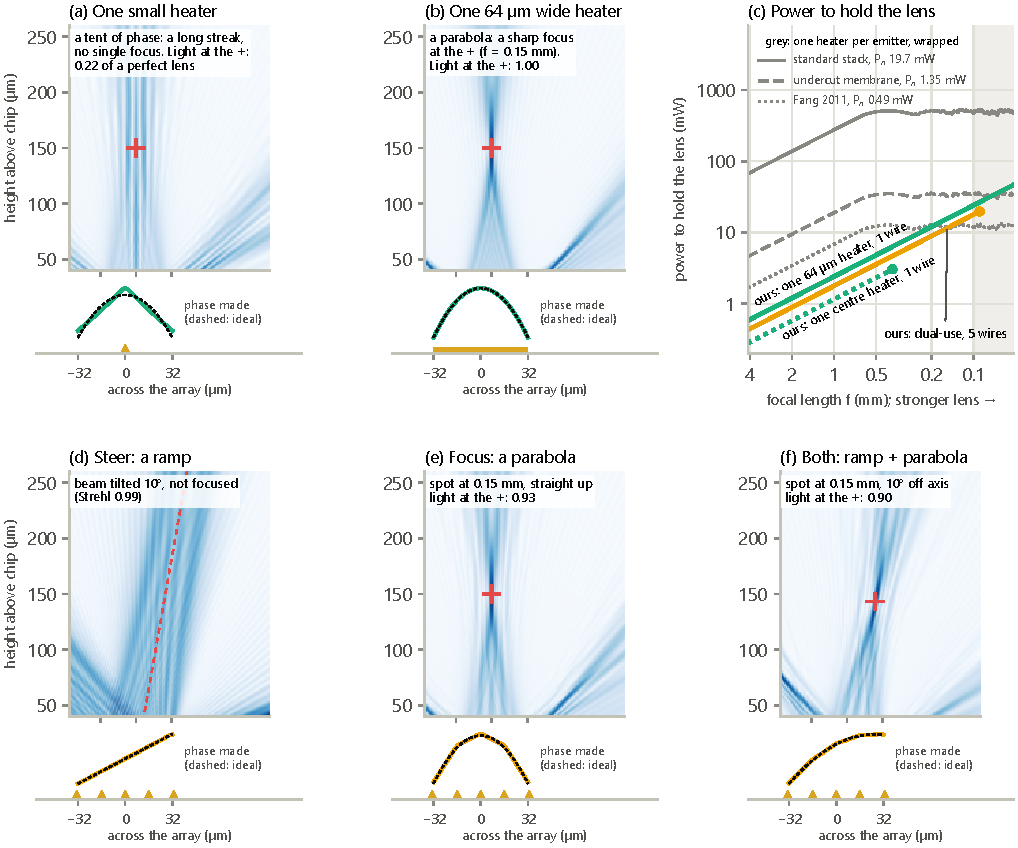
\includegraphics[width=\linewidth]{rep_lens}
  \caption{The thermal lens on the \stack{undercut} membrane. (a,~b,~d--f)~Two-dimensional scalar simulation of the
  light above the array (square-root intensity scale); the cross marks the focus of a perfect lens, and the strip
  below each map shows the phase produced (solid) against the target (dashed), with the heaters in gold.
  (a)~One narrow centre heater and (b)~one \qty{64}{\micro\metre} heater, both asked for $f=\qty{0.15}{\milli\metre}$.
  (c)~Power to hold a lens against focal length; grey, one isolated heater per emitter with wrapped phases at three
  values of $\Ppi$; shaded, $f<\qty{0.1}{\milli\metre}$, where the paraxial form is approximate. (d--f)~The five-heater
  layout steering to \ang{10}, focusing, and both at once. The faint diagonal streaks are grating lobes.}
  \label{fig:lens}
\end{figure}

\subsection{Nonlinearity at high temperature}
\label{sec:nonlinear}

Because the ramp cannot be wrapped, the hottest core is about \qty{62}{\kelvin} above ambient at \ang{10}, beyond the
range in which the linear model is accurate to \qty{1}{\percent} (about \qty{30}{\kelvin}). With temperature-dependent
conductivities the true rise falls below the linear prediction by \qty{2.4}{\percent} at \qty{80}{\kelvin} and
\qtyrange{6}{7}{\percent} at \qty{185}{\kelvin} (\cref{fig:nonlinear}a), because oxide, which carries the heat,
conducts better when hot.

This departure follows a simple law. For conductivity $k=k_0(1+\beta\Delta T)$, the Kirchhoff transform
$\vartheta=\Delta T+\beta\Delta T^2/2$ satisfies $k_0\nabla\vartheta=k\nabla T$ and hence obeys the linear equation with
the same sources and boundary values~\cite{carslaw1959}. The linear model therefore gives $\vartheta$ exactly, and to
first order
\begin{equation}
  \Delta T \;=\; \vartheta - a\,\vartheta^{2}, \qquad a=\beta/2 .
  \label{eq:kirchhoff}
\end{equation}
With $a=\qty{3.0e-4}{\per\kelvin}$ on the membrane and \qty{3.5e-4}{\per\kelvin} on the \stack{standard} stack,
\cref{eq:kirchhoff} reproduces every nonlinear profile to within \qty{0.25}{\percent} of the peak, and the two-heater
runs to \qty{0.14}{\percent}. Any drive can therefore be evaluated by superposing linearly and applying
\cref{eq:kirchhoff}. Silicon's thermo-optic coefficient also rises with temperature~\cite{cocorullo1999}, which acts in
the opposite direction; its relative rate $b$ could not be confirmed from the original paper and is bracketed between
0 and \qty{1.4e-3}{\per\kelvin}.

When the heater powers are fitted to the true, nonlinear response, as a calibration on a real device would do, the
beam quality is nearly unchanged (\cref{fig:nonlinear}b). For the \stack{slot} design with \qty{1}{\milli\metre}
heaters, $S$ at \ang{10} is \numrange{0.95}{0.97} against \num{0.96} for the linear model, and the drive differs from
the linear one by about \qty{2}{\percent}. At \ang{20} (\qty{120}{\kelvin}) $S$ is \numrange{0.81}{0.89}. The
nonlinearity is therefore a calibration matter, not a limit on the design, up to about \ang{20} with
\qty{1}{\milli\metre} heaters; longer heaters reduce the temperature in proportion.

\begin{figure}[htbp]
  \centering
  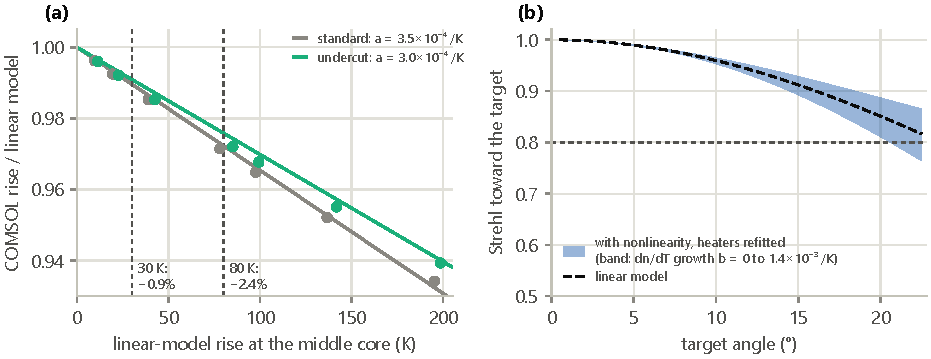
\includegraphics[width=\linewidth]{rep_nonlinear}
  \caption{Nonlinearity. (a)~True temperature rise divided by the linear prediction, with the law of
  \cref{eq:kirchhoff}. (b)~Strehl ratio of the \stack{slot} design (\qty{1}{\milli\metre} heaters) with the heater
  powers fitted to the nonlinear response, for the range of $b$, against the linear model. The hottest core reaches
  \qty{30}{\kelvin} at \ang{4.8} and \qty{80}{\kelvin} at \ang{13.2}.}
  \label{fig:nonlinear}
\end{figure}

\subsection{The grating axis}
\label{sec:gratingaxis}

Along the waveguides the emission angle follows the grating equation,
\begin{equation}
  \sin\theta_y \;=\; \neff^{\mathrm{g}} - \frac{\lambda}{\Lambda},
  \label{eq:grating}
\end{equation}
with $\Lambda$ the period and $\neff^{\mathrm g}$ the effective index of the grating section. The grating model gives
\ang{9.64} at the design point and rates of $+\ang{1.90}$ per \qty{10}{\nano\metre} of period, $+\ang{1.16}$ per
\qty{100}{\kelvin}, and $-\ang{0.150}$ per nanometre of wavelength after correction for the strip's group index
(\cref{fig:grating}); all \num{18} runs lie within \ang{0.03} of \cref{eq:grating}. Tuning the laser from
\qtyrange{1500}{1600}{\nano\metre} sweeps the beam by about \ang{15} along the grating, which together with the
\ang{\pm 22.8} across the array gives a two-dimensional field of view. The temperature sensitivity is also why the
heaters sit before the gratings: steering heaters over a grating would be limited to its \qty{110}{\micro\metre}
emission length, requiring about \qty{370}{\kelvin} at \ang{10} and tilting the beam by about \ang{4} along the
grating.

\begin{figure}[htbp]
  \centering
  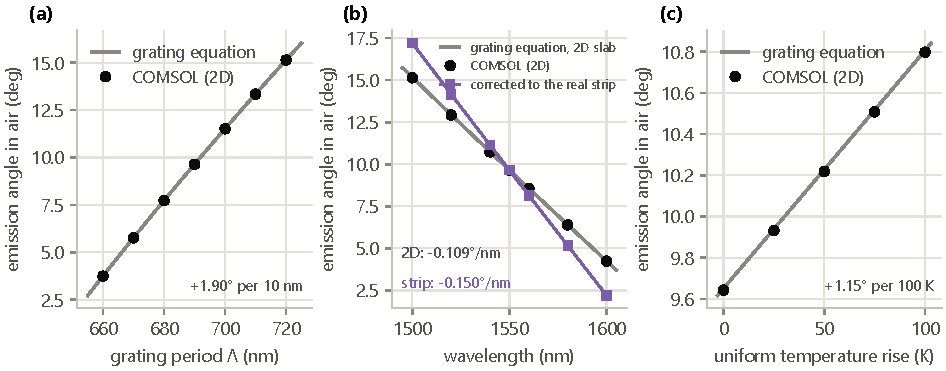
\includegraphics[width=\linewidth]{rep_grating}
  \caption{Grating model: emission angle against (a)~period, (b)~wavelength, with the correction for the strip's
  group index, and (c)~temperature. Grey lines are the grating equation with nothing fitted.}
  \label{fig:grating}
\end{figure}

% =====================================================================================
\section{Discussion}
\label{sec:discussion}
% =====================================================================================

\subsection{Comparison with published devices}
\label{sec:compare}

Our results are simulated and the published ones are measured unless marked otherwise. Steering power is compared at
a fixed angle (\ang{10}) and scaled to $N=33$, because a wrapped array draws nearly the same power at any angle and
power per degree would favour it at large angles.

\paragraph{Few-wire steering.} The directly comparable designs are those that also steer with a few signals
(\cref{tab:fewwire}). Measured cascaded arrays at our pitch need about \qtyrange{12}{17}{\mWdeg} when scaled to
\num{33} emitters; the \stack{slot} and \stack{vacuum} designs need \num{1.38} and \qty{0.53}{\mWdeg},
\numrange{10}{30} times less. The cascaded arrays are much faster (\qty{100}{\kilo\hertz} bandwidth~\cite{yaacobi2014}
against our \qtyrange{50}{190}{\hertz} with plain steps), but their heated stages are micrometres long and run near
\qty{500}{\celsius}, and their series feed accumulates loss and error along the bus.

\begin{table}[htbp]
  \centering
  \caption{Steering with few control signals. Power per degree of the published arrays is scaled to $N=33$ from the
  reported totals (our estimate).}
  \label{tab:fewwire}
  \footnotesize
  \setlength{\tabcolsep}{4pt}
  \begin{tabularx}{\linewidth}{@{}P{0.18\linewidth}LcP{0.1\linewidth}P{0.1\linewidth}cP{0.11\linewidth}@{}}
    \toprule
    Work & Ramp made by & Wires & Array & Range & \unit{\mWdeg} & Basis \\
    \midrule
    This work, \stack{vacuum} & heat flow across a slotted membrane & 1 & $33\times\qty{2}{\micro\metre}$ &
        \ang{22.8} one way & 0.53 & simulated \\
    This work, \stack{slot} & same, in air & 3 & same & \ang{22.8} one way & 1.38 & simulated \\
    This work, \stack{undercut} & membrane anchored at both walls & 4 & same & \ang{\pm 22.8} & 5.24 & simulated \\
    \addlinespace
    Yaacobi~\cite{yaacobi2014} & cascaded heaters on one bus & 1 & $16\times\qty{2}{\micro\metre}$ & \ang{51} &
        $\approx12$ & measured, scaled \\
    Poulton~\cite{poulton2016} & cascade in three groups & 3 & $50\times\qty{2}{\micro\metre}$ & \ang{46} &
        $\approx17$ & measured, scaled \\
    Van Acoleyen~\cite{vanacoleyen2009} & one triangular electrode & 1 & $16\times\qty{2}{\micro\metre}$ & \ang{2.3}
        & $\propto N^2$ & measured \\
    Hosseini~\cite{hosseini2025} & meander overlap (SiN, \qty{525}{\nano\metre}) & 4 & 16 & \ang{\pm 5.1} & --- &
        measured \\
    \bottomrule
  \end{tabularx}
\end{table}

\paragraph{One heater per emitter.} Against arrays of the best individual phase shifters the result depends on the
device (\cref{sec:power}): at \ang{10} the \stack{slot} design equals \num{33} single-pass suspended
heaters~\cite{fang2011} and the \stack{vacuum} design needs \num{3.6} times more than \num{33} folded record
shifters~\cite{lu2015}. These arrays have not been built; the record devices are large (a \qty{6}{\milli\metre}
folded arm~\cite{lu2015}) and would need a fan-in and \num{33} drivers. Measured thermo-optic OPAs draw
\qtyrange{3.7}{9.4}{\milli\watt} per element~\cite{miller2020,phare2018}, against our
\qtyrange{0.16}{0.42}{\milli\watt}, but their totals include the power used to cancel fabrication errors, which our
design replaces with a trim.

\paragraph{Lenses.} The two measured few-heater lenses found cost about \qty{40}{\milli\watt\per\rad} (shaped heaters
on a silicon slab metalens~\cite{liu2023}) and \qtyrange{70}{110}{\milli\watt\per\rad} (meanders in silicon
nitride~\cite{hosseini2025}), converted by us from the reported focal shifts and good to about a factor of two. Ours,
at about \qty{1}{\milli\watt\per\rad}, is \numrange{30}{100} times lower. Most of this difference is due to the
platform: those devices sit on solid substrates, and silicon nitride's thermo-optic coefficient is about seven times
smaller than silicon's. The metalens is about ten times faster.

\Cref{tab:scoreboard} summarises the comparison.

\begin{table}[htbp]
  \centering
  \caption{Summary of the comparison. Ours: two-dimensional simulation. Theirs: measured, or, where marked $\dagger$,
  our estimate for \num{33} copies of a measured device.}
  \label{tab:scoreboard}
  \footnotesize
  \begin{tabularx}{\linewidth}{@{}P{0.17\linewidth}P{0.25\linewidth}LP{0.2\linewidth}@{}}
    \toprule
    Metric & This work & Best published & Outcome \\
    \midrule
    Few-wire steering power & \qtyrange{0.53}{1.38}{\mWdeg}, 1--3 wires & \qtyrange{12}{17}{\mWdeg}, 1--3
        wires~\cite{yaacobi2014,poulton2016} & $10$--$30\times$ lower \\
    Power at \ang{10} & \qty{5.3}{\milli\watt} (\stack{vacuum}), \qty{13.8}{\milli\watt} (\stack{slot}) &
        \qty{1.5}{\milli\watt}$^\dagger$~\cite{lu2015}; \qty{14.4}{\milli\watt}$^\dagger$~\cite{fang2011} &
        $3.6\times$ higher than the record; equal to single-pass \\
    Tunable lens & \qtyrange{0.9}{1.2}{\milli\watt\per\rad}, 1--5 wires & \qtyrange{40}{110}{\milli\watt\per\rad}
        (est.)~\cite{liu2023,hosseini2025} & $30$--$100\times$ lower \\
    Speed, \ang{0}$\to$\ang{10} & \qtyrange{2}{9}{\milli\second} plain; \qtyrange{0.16}{1.4}{\milli\second}
        with pre-emphasis & \qty{2}{\micro\second}~\cite{jacques2019} to \qty{144}{\micro\second}~\cite{fang2011}
        per device & slower; power $\times$ time $1.2$--$16\times$ higher with pre-emphasis \\
    Field of view & \ang{\pm 22.8} (one way for \stack{slot}, \stack{vacuum}) & \ang{51} at the same
        pitch~\cite{yaacobi2014} & comparable within pitch class \\
    Calibration & one trim, then a linear fit and a gain curve & a search per beam~\cite{lian2024} & simpler, given
        the trim \\
    Independent errors & not correctable; trim required & fully corrected & worse \\
    Patterns & ramp and dome only & arbitrary & worse \\
    \bottomrule
  \end{tabularx}
\end{table}

\subsection{Agreement with real devices}
\label{sec:fidelity}

The single-heater versions of our thermal model agree with measured devices. Our \stack{standard} heater has
$\Ppi=\qty{19.7}{\milli\watt}$, against \qtyrange{22.8}{29.2}{\milli\watt} measured for TiN and doped-silicon
heaters~\cite{jacques2019}; our \stack{undercut} heater has \qty{1.35}{\milli\watt} and \qty{1.6}{\milli\second},
against \qty{1.07}{\milli\watt} and \qtyrange{1.3}{1.9}{\milli\second} for a foundry undercut~\cite{parsons2025}.
Published comparisons of simulated and measured thermo-optic devices agree to about $\pm\qty{15}{\percent}$ for
conventional heaters and within a factor of \numrange{0.67}{1.5} for undercut structures with idealised geometry. A
real back-end stack would also add oxide above the heater, increasing $\kt$ and the power by \numrange{1.5}{1.9}
times. A fabricated \stack{slot} design would therefore need roughly \qtyrange{9}{40}{\milli\watt} at \ang{10}, and a
\stack{vacuum} design \qtyrange{3.5}{15}{\milli\watt} (our estimate), still several times below the measured few-wire
arrays. The structure itself, a single \qty{80}{\micro\metre} membrane under a whole array, has not been fabricated;
published undercuts isolate single devices with undercuts of order \qty{10}{\micro\metre}~\cite{parsons2025}.
The \stack{vacuum} design also needs a sealed package. Gas conduction across the \qty{15}{\micro\metre} cavity
falls only once the mean free path approaches the gap, and a simple kinetic estimate puts the required pressure
near \qty{100}{\pascal}; no thermo-optic device has, to our knowledge, been measured in vacuum.

\subsection{Limitations}
\label{sec:limitations}

\Cref{tab:limits} lists the limitations, the claims they affect and how each could be resolved. The most important is
that all thermal results are two-dimensional: a finite heater loses some heat through the cavity ends (an estimated
\qtyrange{5}{8}{\percent} more power for \qty{1}{\milli\metre} heaters), and heat conducted along the waveguides could
reach the gratings. In addition, the \stack{slot} and \stack{vacuum} designs steer in one direction only, and the
design does not scale unchanged to large apertures: at \num{128} emitters the hot end would reach about
\qty{250}{\kelvin} at \ang{10}, and settling would be about \num{16} times slower.

\begin{table}[htbp]
  \centering
  \caption{Limitations.}
  \label{tab:limits}
  \footnotesize
  \begin{tabularx}{\linewidth}{@{}P{0.24\linewidth}P{0.22\linewidth}LP{0.18\linewidth}@{}}
    \toprule
    Limitation & Affects & Expected size & Resolved by \\
    \midrule
    2D model; no heater or cavity ends & all powers; grating temperature & $+$\qtyrange{5}{8}{\percent} power (est.);
        grating heating unknown & 3D thermal model \\
    No fabricated device & absolute values & $\times0.67$--$1.5$; $\times1.5$--$1.9$ for a real stack & test chip \\
    Idealised release and \qty{2}{\micro\metre} slot & \stack{slot} power & a wider slot and deeper cavity help &
        realistic-stack model \\
    Mechanics not modelled & membrane feasibility & buckling margin, slot-edge curl unknown & thermo-mechanical
        model \\
    Vacuum operation unprecedented & \stack{vacuum} results & --- & measurement against pressure \\
    Emitters identical and independent & far-field model & small ($L_c=\qty{2.2}{\metre}$) & 3D full-wave model \\
    Static trim assumed & beam quality beyond small angles & $S\approx0.78$ untrimmed at \ang{10} & trim shown on
        an OPA \\
    Silicon's $\mathrm{d}n/\mathrm{d}T$ growth unconfirmed & sign of pointing error & $\pm\ang{0.25}$ at \ang{10}
        before gain correction & coefficients of Ref.~\cite{cocorullo1999} \\
    Kernel-shape errors not modelled & calibration & expected to rescale the ramp & sensitivity runs \\
    One-way steering (\stack{slot}, \stack{vacuum}) & field of view & half the field, or twice the power &
        two-sided layout \\
    \bottomrule
  \end{tabularx}
\end{table}

\subsection{Applications and further work}

The design is a low-wire, low-power, slow actuator for smooth phase profiles over a small aperture. It suits tasks
that need a ramp or a parabola of variable strength at rates below about \qty{100}{\hertz}, such as tip-tilt
correction behind a telescope in ground-level free-space links, where loop bandwidths of \qtyrange{1}{70}{\hertz} are
required~\cite{frost2024}, coarse beam acquisition and variable focus. It does not suit LiDAR scanning, which needs
\qtyrange{10}{100}{\kilo\hertz}, or adaptive optics, which needs arbitrary phase profiles.

The next steps, all specified as COMSOL models, are: a three-dimensional model of a finite heater and cavity including
the gratings; a model with a realistic back-end stack, a wider release slot and an isotropic cavity; the
thermo-mechanical bow of the slotted membrane; kernel sensitivities to fabrication variations; and a two-sided slot
layout.

% =====================================================================================
\section{Conclusion}
\label{sec:conclusion}
% =====================================================================================

This report examined whether the heat that spreads between the waveguides of a thermo-optic phased array, normally
suppressed, can be used to steer it. In simulation it can, provided the structure makes the steady temperature
profile take the shape of the required phase.

Heat spreading acts as a spatial low-pass filter, and the ratio of spreading length to pitch determines what a few
heaters can do. On a standard stack ($\Lth/d\approx1.7$) a few heaters cannot steer. On a membrane undercut beneath
the array ($\Lth/d\approx10$) three or four heaters steer at about \qty{4.9}{\mWdeg}, but most of the edge heater's
power flows into the nearby wall. A slot past that heater removes this path, so the heat crosses the array and the
temperature becomes a linear ramp. Three heaters then steer \num{33} emitters across \ang{22.8} at \qty{1.38}{\mWdeg}
in air, and one heater does so at \qty{0.53}{\mWdeg} in vacuum, within \qty{5}{\percent} of a conduction limit that is
independent of the number of emitters. Uniform heating of a membrane between two walls gives a parabolic profile and
hence a one-wire tunable lens at about \qty{1}{\milli\watt\per\rad}.

The three capabilities of individual control are lost to a quantified extent. Without phase wrapping the power grows
with angle, the hottest waveguide is about \qty{62}{\kelvin} above ambient at \ang{10}, and a \ang{10} step takes
\qtyrange{2}{9}{\milli\second} with a plain drive, or \qtyrange{0.16}{1.4}{\milli\second} when each heater's
drive is shaped in time, provided the thermal time scale is known to a few per cent. Only two to four phase patterns are usable. Independent fabrication errors cannot be
corrected, so a one-time static trim is required, after which calibration reduces to a linear fit and a gain curve.

Compared with published devices, the design needs \numrange{10}{30} times less power than measured few-wire arrays and
\numrange{30}{100} times less than measured few-heater lenses, and is correspondingly slower. It is not the
lowest-power phased array: \num{33} of the best folded phase shifters would hold \ang{10} with about a quarter of the
power, but would require \num{33} wires and a fan-in.

These results rest on two-dimensional finite-element models that pass their convergence, conservation and consistency
checks, and on an array model that reproduces its analytic limits. They have not been tested in three dimensions or on
a fabricated device. Within these limits, thermal crosstalk can be used as a resource for the smooth phase profiles
that steering and focusing require, at a quantified cost in speed and control.

\section*{Data and code availability}
\addcontentsline{toc}{section}{Data and code availability}
The COMSOL exports, the Python code, the result tables and the figure scripts are available at
\url{https://github.com/shanmehta2210/Diffusion_in_Waveguides}.


% ---------- back matter ----------------------------------------------------------------
\bibliographystyle{unsrtnat}
\bibliography{references}



\end{document}
